\documentclass[11pt,letterpaper,oneside]{report}
\usepackage[T1]{fontenc}
\usepackage[utf8]{inputenc}
\usepackage[margin=1in]{geometry}
\usepackage{amsmath,amssymb}
\usepackage{booktabs}
\usepackage{tikz}
\usetikzlibrary{arrows.meta,calc}
\definecolor{robotframe}{RGB}{180,55,35}
\definecolor{sensorframe}{RGB}{30,105,155}
\tikzset{axis/.style={-{Stealth},thick},projection/.style={dashed,thin},
 every node/.style={font=\small}}
\usepackage[expansion=false]{microtype}
\usepackage[hidelinks]{hyperref}
\hypersetup{pdftitle={ELE456 Lecture Notes},pdfauthor={Paolo Stegagno}}
\setlength{\parindent}{0pt}
\setlength{\parskip}{0.55em}
\setcounter{tocdepth}{1}
\newcommand{\R}{\mathbb{R}}
\newcommand{\trans}{^{\mathsf T}}

\title{ELE456\\Lecture Notes}
\author{Lectures by Paolo Stegagno}
\date{Fall 2026}

\begin{document}
\hypersetup{pageanchor=false}
\maketitle
\pagenumbering{roman}
\hypersetup{pageanchor=true}
\chapter*{About these notes}
These notes develop the mathematical foundations of robotics, from linear
algebra to models of robot motion, sensing, and planning. Each chapter introduces
a topic through definitions, explanations, and worked examples. The material
builds progressively, with an emphasis on understanding the assumptions behind
each calculation and interpreting the resulting relationships.

\medskip
\textbf{Preparation.} These notes are prepared with AI assistance from
Paolo Stegagno's lecture transcripts and board material and reviewed by the
instructor. Errors may remain; please report suspected mistakes.

\medskip
\textbf{License.} Copyright \textcopyright\ 2026 Paolo Stegagno, to the extent
copyright applies. Unless otherwise noted, these notes, diagrams, and their
LaTeX/TikZ sources are licensed under
\href{https://creativecommons.org/licenses/by-nc/4.0/}{Creative Commons
Attribution-NonCommercial 4.0 International (CC BY-NC 4.0)}.
Sharing and adaptation are permitted for noncommercial purposes with
appropriate attribution, a license link, and an indication of changes.
Commercial uses outside the license require separate permission.
Uses otherwise permitted by law and public-domain material are unaffected.
The full terms are available at
\url{https://creativecommons.org/licenses/by-nc/4.0/legalcode}.
\tableofcontents
\clearpage
\pagenumbering{arabic}
\chapter{Introduction and linear algebra}
\label{chap:lecture01}

Robotics brings together mathematical models of motion, measurements from
sensors, and algorithms that determine how a robot should act. Describing a
robot's position, relating measurements to its surroundings, and planning its
motion all require a precise mathematical language. Linear algebra provides
many of the tools used to express these relationships.

This chapter introduces matrices and the operations needed to work with them:
addition, multiplication, transposition, and inversion. It then examines
orthogonal matrices, whose inverses can be obtained simply by transposing.
The examples develop two habits that will remain essential throughout the
study of robotics: checking dimensions before performing an operation and
preserving the order of factors in a matrix product.
\section{Matrices and dimensions}

A \emph{matrix} is an array of numbers arranged in rows and columns. Its
dimensions are written as
\[
  \text{number of rows}\times\text{number of columns}.
\]
Consider the matrix
\begin{equation}
 A=\begin{bmatrix}1&2\\3&1\\0&1\end{bmatrix}\in\R^{3\times2}.
 \label{eq:l01-A}
\end{equation}
It has three rows and two columns. In general, $a_{ij}$ denotes the entry in
row $i$, column $j$; for example, $a_{21}=3$ and $a_{32}=1$.

\section{Matrix addition}

Two matrices can be added only if they have the same dimensions. Their entries
are then added in corresponding positions:
\[
 (A+C)_{ij}=a_{ij}+c_{ij}.
\]
Consider two additional matrices,
\[
 B=\begin{bmatrix}1&2\\1&1\end{bmatrix}\in\R^{2\times2},
 \qquad
 C=\begin{bmatrix}0&1\\0&0\\1&0\end{bmatrix}\in\R^{3\times2}.
\]
The sum $A+B$ is undefined because the dimensions differ. The sum $A+C$ is
defined, and its calculation is
\begin{equation}
 A+C
 =\begin{bmatrix}1+0&2+1\\3+0&1+0\\0+1&1+0\end{bmatrix}
 =\begin{bmatrix}1&3\\3&1\\1&1\end{bmatrix}.
\end{equation}
Addition is commutative when defined: $A+C=C+A$.

\section{Matrix multiplication}

\subsection{Dimension rule and row-by-column calculation}
For matrices $M\in\R^{m\times n}$ and $N\in\R^{n\times p}$, the product
$MN$ is defined and has dimensions $m\times p$:
\[
 \underbrace{(m\times n)(n\times p)}_{\text{inner dimensions must match}}
 \quad\longrightarrow\quad m\times p.
\]
The entry in row $i$, column $j$ is the sum of the products of corresponding
entries of row $i$ of $M$ and column $j$ of $N$:
\begin{equation}
 (MN)_{ij}=\sum_{k=1}^{n}m_{ik}n_{kj}.
\end{equation}
Matrix multiplication is therefore a row-by-column operation, rather than
entrywise multiplication.

For the matrices $A$ and $B$ above, the dimensions are
$(3\times2)(2\times2)$, so $AB$ is a $3\times2$ matrix:
\begin{align}
 AB
 &=\begin{bmatrix}1&2\\3&1\\0&1\end{bmatrix}
   \begin{bmatrix}1&2\\1&1\end{bmatrix}\\
 &=\begin{bmatrix}
  1\cdot1+2\cdot1 & 1\cdot2+2\cdot1\\
  3\cdot1+1\cdot1 & 3\cdot2+1\cdot1\\
  0\cdot1+1\cdot1 & 0\cdot2+1\cdot1
 \end{bmatrix}
 =\begin{bmatrix}3&4\\4&7\\1&1\end{bmatrix}.
 \label{eq:l01-AB}
\end{align}

\subsection{The order of the factors matters}
Reversing the factors gives the dimensions $(2\times2)(3\times2)$. The inner
dimensions do not match, so $BA$ is undefined, even though $AB$ exists.

Even when both orders are defined, the results need not agree. With
\[
 E=\begin{bmatrix}1&2\\3&4\end{bmatrix},
\]
direct multiplication gives
\[
 BE=\begin{bmatrix}7&10\\4&6\end{bmatrix},
 \qquad
 EB=\begin{bmatrix}3&4\\7&10\end{bmatrix}.
\]
Thus $BE\ne EB$. Matrix multiplication is not commutative in general. Some
particular matrices do commute, but factors cannot be exchanged without a
reason that applies to the matrices in question.

\section{The transpose}

Transposing a matrix interchanges its rows and columns. In entry notation,
$(M\trans)_{ij}=m_{ji}$. If $M$ has dimensions $m\times n$, then $M\trans$
has dimensions $n\times m$. For the running example,
\begin{equation}
 A\trans=\begin{bmatrix}1&3&0\\2&1&1\end{bmatrix}\in\R^{2\times3}.
\end{equation}

The transpose of a product reverses the order of its factors:
\begin{equation}
 \boxed{(AB)\trans=B\trans A\trans.}
 \label{eq:l01-transpose-product}
\end{equation}
The dimensions provide a quick check. Here $B\trans A\trans$ has dimensions
$(2\times2)(2\times3)$, producing a $2\times3$ matrix as required. The
incorrect expression $A\trans B\trans$ would have dimensions
$(2\times3)(2\times2)$ and is undefined.

Using the matrices defined above, this identity can be verified directly:
\[
 B\trans A\trans
 =\begin{bmatrix}1&1\\2&1\end{bmatrix}
  \begin{bmatrix}1&3&0\\2&1&1\end{bmatrix}
 =\begin{bmatrix}3&4&1\\4&7&1\end{bmatrix}
 =(AB)\trans.
\]
Dimension checks can rule out an invalid expression, but matching dimensions
alone do not prove that an identity is correct.

\section{Identity matrices and inverses}

The identity matrix $I_n$ has ones on its main diagonal and zeros elsewhere.
For a square matrix $M\in\R^{n\times n}$, an inverse $M^{-1}$ satisfies
\begin{equation}
 MM^{-1}=M^{-1}M=I_n.
\end{equation}
This ordinary, two-sided inverse is defined only for square matrices, and not
every square matrix has one. The condition for invertibility is
\begin{equation}
 \boxed{\det(M)\ne0.}
\end{equation}
A square matrix with zero determinant is called \emph{singular}.

\subsection{A one-by-one example}
For $H=\begin{bmatrix}5\end{bmatrix}$, the inverse is
$H^{-1}=\begin{bmatrix}1/5\end{bmatrix}$, since
\[
 HH^{-1}=H^{-1}H=\begin{bmatrix}1\end{bmatrix}=I_1.
\]
This is the familiar reciprocal operation for a nonzero scalar.

\subsection{A diagonal example and its determinant}
The second example is
\[
 G=\begin{bmatrix}1&0\\0&2\end{bmatrix},
 \qquad
 G^{-1}=\begin{bmatrix}1&0\\0&1/2\end{bmatrix}.
\]
Multiplying verifies the inverse:
\[
 GG^{-1}
 =\begin{bmatrix}
 1\cdot1+0\cdot0&1\cdot0+0\cdot\tfrac12\\
 0\cdot1+2\cdot0&0\cdot0+2\cdot\tfrac12
 \end{bmatrix}
 =\begin{bmatrix}1&0\\0&1\end{bmatrix}=I_2.
\]
The reverse product also equals $I_2$. For a general $2\times2$ matrix,
\[
 \det\begin{bmatrix}a&b\\c&d\end{bmatrix}=ad-bc.
\]
Hence $\det(G)=1\cdot2-0\cdot0=2\ne0$, as required. Reciprocating the
diagonal entries works here because $G$ is diagonal with nonzero diagonal
entries; matrix inversion is not generally an entrywise reciprocal operation.

\section{Orthogonal matrices}

A real square matrix $L$ is \emph{orthogonal} if its inverse equals its
transpose:
\begin{equation}
 \boxed{L^{-1}=L\trans.}
\end{equation}
Equivalently, $LL\trans=L\trans L=I$. This gives a practical way to check
orthogonality: form the transpose, multiply, and verify the identity matrix.
For an orthogonal matrix, an inverse can be obtained by transposing instead of
performing a general inverse calculation.

\subsection{Verifying orthogonality}
Consider
\[
 L=\begin{bmatrix}
 \tfrac12&\tfrac{\sqrt3}{2}\\
 -\tfrac{\sqrt3}{2}&\tfrac12
 \end{bmatrix},
 \qquad
 L\trans=\begin{bmatrix}
 \tfrac12&-\tfrac{\sqrt3}{2}\\
 \tfrac{\sqrt3}{2}&\tfrac12
 \end{bmatrix}.
\]
Their product is
\begin{align}
 LL\trans
 &=\begin{bmatrix}
 \tfrac14+\tfrac34&-\tfrac{\sqrt3}{4}+\tfrac{\sqrt3}{4}\\
 -\tfrac{\sqrt3}{4}+\tfrac{\sqrt3}{4}&\tfrac34+\tfrac14
 \end{bmatrix}\\
 &=\begin{bmatrix}1&0\\0&1\end{bmatrix}=I_2.
\end{align}
Thus $L$ is orthogonal and the displayed $L\trans$ is its inverse.

\subsection{The trigonometric pattern}
The preceding example belongs to the family
\begin{equation}
 Q(\theta)=\begin{bmatrix}
 \sin\theta&\cos\theta\\
 -\cos\theta&\sin\theta
 \end{bmatrix}.
 \label{eq:l01-Q}
\end{equation}
Multiplying by the transpose gives
\begin{align*}
 Q(\theta)Q(\theta)\trans
 &=\begin{bmatrix}
 \sin^2\theta+\cos^2\theta & -\sin\theta\cos\theta+\cos\theta\sin\theta\\
 -\cos\theta\sin\theta+\sin\theta\cos\theta & \cos^2\theta+\sin^2\theta
 \end{bmatrix}\\
 &=I_2.
\end{align*}
The identity $\sin^2\theta+\cos^2\theta=1$ makes this family orthogonal for
every real $\theta$.

The numerical example corresponds to $L=Q(\pi/6)$, since
$\sin(\pi/6)=1/2$ and $\cos(\pi/6)=\sqrt3/2$. An equivalent
parameterization uses cosine on the diagonal:
\[
 P(\varphi)=\begin{bmatrix}
 \cos\varphi&\sin\varphi\\
 -\sin\varphi&\cos\varphi
 \end{bmatrix}.
\]
The relation $Q(\theta)=P(\pi/2-\theta)$ follows from the complementary-angle
identities. Thus the same numerical matrix is $L=P(\pi/3)$. In either
parameterization, orthogonality follows from the same trigonometric identity.
Such matrices provide a foundation for describing changes of orientation
in robotics.
\section{Key identities}
For matrices of compatible dimensions, the operations developed in this
chapter can be collected as follows:
\begin{center}
\begin{tabular}{ll}
\toprule
Operation or property & Rule \\
\midrule
Addition & $(M+N)_{ij}=m_{ij}+n_{ij}$ \\
Multiplication & $(MN)_{ij}=\sum_{k=1}^{n}m_{ik}n_{kj}$ \\
Transpose & $(M\trans)_{ij}=m_{ji}$ \\
Transpose of a product & $(MN)\trans=N\trans M\trans$ \\
Inverse & $MM^{-1}=M^{-1}M=I$ \\
Invertibility of a square matrix & $\det(M)\ne0$ \\
Orthogonality & $M^{-1}=M\trans$ \\
\bottomrule
\end{tabular}
\end{center}
In the multiplication formula, $n$ is the number of columns of $M$ and the
number of rows of $N$. Addition requires equal dimensions, whereas a product
requires only that these inner dimensions match. Inverse and orthogonality
conditions apply to square matrices. These distinctions determine which
algebraic manipulations are valid before any numerical calculation begins.

\clearpage
\section{Additional exercises}
Show your calculations and justify each conclusion. Check dimensions before
performing an operation. These exercises can be completed by hand.

\begin{enumerate}
\item \textbf{Dimensions and valid operations.}
Let $A\in\R^{3\times2}$, $B\in\R^{2\times3}$, and
$C\in\R^{3\times3}$. Determine which expressions are defined and give the
dimensions of each valid result:
\[
 A+B,\qquad AB,\qquad BA,\qquad CA,\qquad AC,\qquad
 A\trans+C,\qquad B+A\trans.
\]

\item \textbf{Addition and multiplication.}
Consider
\[
 M=\begin{bmatrix}2&-1\\0&3\end{bmatrix},\qquad
 N=\begin{bmatrix}1&2\\-1&0\end{bmatrix},\qquad
 v=\begin{bmatrix}1\\-2\end{bmatrix}.
\]
Compute $M+N$, $MN$, $NM$, and $Mv$. Do $M$ and $N$ commute?
Verify numerically that $(M+N)v=Mv+Nv$.

\item \textbf{Transposing a product.}
Let
\[
 U=\begin{bmatrix}1&0&-1\\2&1&3\end{bmatrix},\qquad
 V=\begin{bmatrix}1&2\\0&-1\\2&0\end{bmatrix}.
\]
Compute $UV$ and $(UV)\trans$, then independently compute
$V\trans U\trans$ and compare the results. Is $U\trans V\trans$
defined? Explain why it cannot equal $(UV)\trans$ in this example.

\item \textbf{Determinants and inverses.}
For
\[
 D=\begin{bmatrix}4&0\\0&-2\end{bmatrix},\qquad
 F=\begin{bmatrix}1&2\\2&4\end{bmatrix},\qquad
 K=\begin{bmatrix}2&1\\1&1\end{bmatrix},
\]
use determinants to decide which matrices are invertible. Find $D^{-1}$.
Verify that $\begin{bmatrix}1&-1\\-1&2\end{bmatrix}$ is the inverse of
$K$ by multiplying in both orders.

\item \textbf{Testing orthogonality.}
Consider
\[
 R=\begin{bmatrix}\tfrac35&-\tfrac45\\[2pt]\tfrac45&\tfrac35\end{bmatrix},
 \qquad S=\begin{bmatrix}1&0\\0&-1\end{bmatrix},
 \qquad T=\begin{bmatrix}1&1\\0&1\end{bmatrix}.
\]
Test each matrix for orthogonality using its transpose. For each orthogonal
matrix, write its inverse. Is an invertible matrix necessarily orthogonal?
Support your answer with one of these examples.

\item \textbf{A product of orthogonal matrices.}
Suppose $P$ and $Q$ are real orthogonal $n\times n$ matrices. Use the
transpose-of-a-product rule to show that $(PQ)(PQ)\trans=I_n$.
Deduce that $PQ$ is orthogonal and express $(PQ)^{-1}$ in terms of
$P\trans$ and $Q\trans$, paying attention to their order.
\end{enumerate}

\chapter{Reference frames and planar rotations}
\label{chap:lecture02}

A robot must relate what its sensors observe to a description of the surrounding
world. An obstacle may be directly ahead of the robot, yet lie in a different
direction when described on a map. Neither description is ambiguous once the
reference frame is specified. The task is to express the same geometric point
in different coordinate systems.

This chapter develops that change of coordinates for planar frames with a
common origin. Their relative orientation is described by one angle, or
equivalently by a rotation matrix. The matrix formulation makes it possible to
transform coordinates, reverse a transformation, and compose transformations
through several frames using the linear algebra of Chapter~\ref{chap:lecture01}.

\section{Coordinates depend on a reference frame}
A planar Cartesian reference frame consists of an origin and two perpendicular
unit directions, denoted $\boldsymbol{x}$ and $\boldsymbol{y}$. A world frame
$W$ provides a fixed reference for a map, while a robot frame $R$ is attached
to the robot. A sensor can have its own frame $S$.

\begin{figure}[htbp]
\centering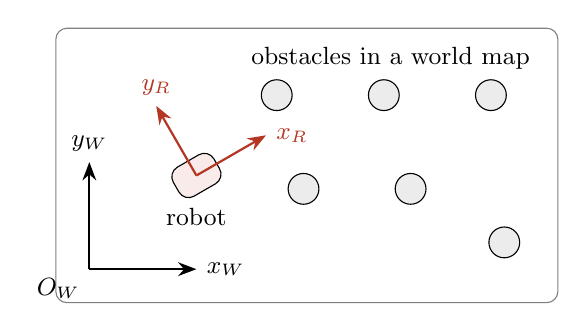
\begin{tikzpicture}[scale=0.85]
\draw[rounded corners,gray] (-.5,-.5) rectangle (7,3.6);
\foreach \x/\y in {2.8/2.6,4.4/2.6,6/2.6,3.2/1.2,4.8/1.2,6.2/.4}
  \draw[fill=gray!15] (\x,\y) circle (.23);
\draw[axis] (0,0)--(1.6,0) node[right] {$x_W$};
\draw[axis] (0,0)--(0,1.6) node[above] {$y_W$};
\node[below left] at (0,0) {$O_W$};
\begin{scope}[shift={(1.6,1.4)},rotate=30]
\draw[fill=robotframe!10,rounded corners] (-.35,-.25) rectangle (.35,.25);
\draw[axis,robotframe] (0,0)--(1.2,0) node[right] {$x_R$};
\draw[axis,robotframe] (0,0)--(0,1.2) node[above] {$y_R$};
\end{scope}
\node[below] at (1.6,1.05) {robot};
\node at (4.5,3.15) {obstacles in a world map};
\end{tikzpicture}

\caption{A map and a robot use different reference frames. In a general setting
their origins and orientations both differ.}
\label{fig:l02-map}
\end{figure}

If the robot's $x_R$ axis points forward and $y_R$ points left, an obstacle one
unit ahead has robot coordinates $[1\;0]\trans$. An obstacle one unit to the
left has coordinates $[0\;1]\trans$. These descriptions alone do not specify
where the obstacles belong on the world map; the relation between the frames
is also needed.

\subsection{Notation and the common-origin assumption}
Let $B$ denote a geometric point. Its coordinates are column vectors,
\begin{equation}
 B^W=\begin{bmatrix}x_B^W\\y_B^W\end{bmatrix},\qquad
 B^R=\begin{bmatrix}x_B^R\\y_B^R\end{bmatrix}.
\end{equation}
The superscript states the frame in which the coordinates are expressed.
The point $B$ does not change when its coordinate description changes.

For now, assume that $W$ and $R$ share an origin $O$ and have the same
orientation convention for their axes. Let $\theta=\theta_R^W$ be the signed
angle from $x_W$ to $x_R$, positive counterclockwise. Only a rotation separates
the two frames. Figure~\ref{fig:l02-coordinates} shows how projections onto
their axes produce different coordinates for the same point.

\begin{figure}[htbp]
\centering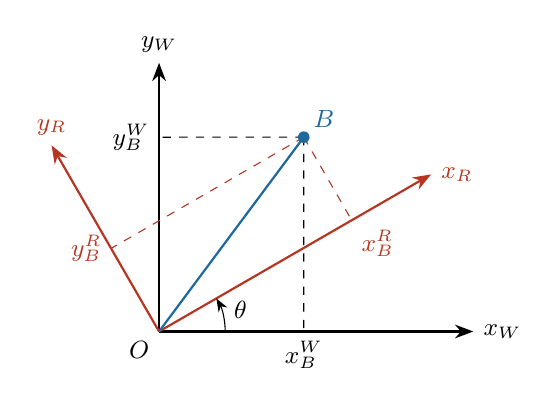
\begin{tikzpicture}[scale=1.05]
\coordinate (B) at (1.75,2.35);
\draw[axis] (0,0)--(3.8,0) node[right] {$x_W$};
\draw[axis] (0,0)--(0,3.25) node[above] {$y_W$};
\draw[axis,robotframe] (0,0)--(30:3.8) node[right] {$x_R$};
\draw[axis,robotframe] (0,0)--(120:2.6) node[above] {$y_R$};
\draw[projection] (B)--(1.75,0) node[below] {$x_B^W$};
\draw[projection] (B)--(0,2.35) node[left] {$y_B^W$};
\coordinate (X) at ({2.69054*cos(30)},{2.69054*sin(30)});
\coordinate (Y) at ({1.16016*cos(120)},{1.16016*sin(120)});
\draw[projection,robotframe] (B)--(X) node[below right] {$x_B^R$};
\draw[projection,robotframe] (B)--(Y) node[left] {$y_B^R$};
\draw[thick,sensorframe] (0,0)--(B);
\fill[sensorframe] (B) circle (2pt) node[above right] {$B$};
\draw[-{Stealth}] (.8,0) arc (0:30:.8);
\node at (15:1.02) {$\theta$};
\node[below left] at (0,0) {$O$};
\end{tikzpicture}

\caption{A point expressed in two frames with a common origin. Black axes
belong to $W$ and red axes to $R$; dashed lines give the coordinate projections.}
\label{fig:l02-coordinates}
\end{figure}

\section{Constructing the rotation matrix}
\subsection{The columns are the rotated basis vectors}
The direction $\boldsymbol{x}_R$ makes angle $\theta$ with $x_W$. Because it
is a unit vector, its components in the world frame are
\begin{equation}
 [\boldsymbol{x}_R]^W=\begin{bmatrix}\cos\theta\\\sin\theta\end{bmatrix}.
\end{equation}
The direction $\boldsymbol{y}_R$ is a further $\pi/2$ counterclockwise, so
\begin{equation}
 [\boldsymbol{y}_R]^W
 =\begin{bmatrix}\cos(\theta+\pi/2)\\\sin(\theta+\pi/2)\end{bmatrix}
 =\begin{bmatrix}-\sin\theta\\\cos\theta\end{bmatrix}.
\end{equation}
Here brackets with a superscript mean the components of a geometric vector
in the indicated frame. The negative sign in the first component of
$[\boldsymbol{y}_R]^W$ is essential: for a small positive angle, $y_R$
points to the left of $y_W$.

\begin{figure}[htbp]
\centering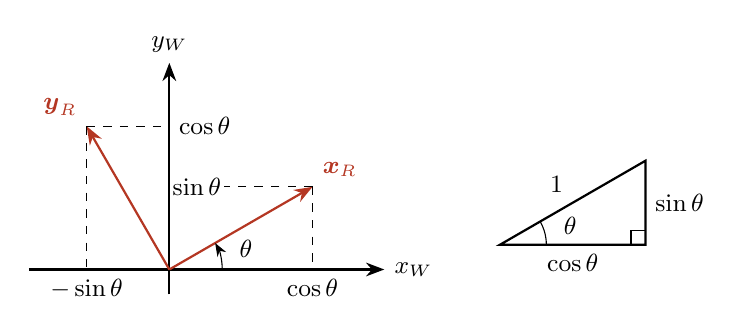
\begin{tikzpicture}[scale=2.1]
\draw[axis] (-.85,0)--(1.3,0) node[right] {$x_W$};
\draw[axis] (0,-.15)--(0,1.25) node[above] {$y_W$};
\draw[axis,robotframe] (0,0)--(30:1) node[above right] {$\boldsymbol{x}_R$};
\draw[axis,robotframe] (0,0)--(120:1) node[above left] {$\boldsymbol{y}_R$};
\draw[projection] (30:1)--({cos(30)},0) node[below] {$\cos\theta$};
\draw[projection] (30:1)--(0,.5) node[right,fill=white,inner sep=1pt] {$\sin\theta$};
\draw[projection] (120:1)--(-.5,0) node[below] {$-\sin\theta$};
\draw[projection] (120:1)--(0,{sin(120)}) node[right] {$\cos\theta$};
\draw[-{Stealth}] (.32,0) arc (0:30:.32);
\node at (15:.48) {$\theta$};
\begin{scope}[shift={(2,0.15)},scale=.8]
\draw[thick] (0,0)--(1.1,0)--(1.1,.635)--cycle;
\node[below] at (.55,0) {$\cos\theta$};
\node[right] at (1.1,.32) {$\sin\theta$};
\node[above left] at (.55,.32) {$1$};
\draw (.35,0) arc (0:30:.35);
\node at (15:.55) {$\theta$};
\draw (.99,0)--(.99,.11)--(1.1,.11);
\end{scope}
\end{tikzpicture}

\caption{Components of the robot's unit basis vectors in the world frame.
The right triangle explains the sine and cosine components of $\boldsymbol{x}_R$.}
\label{fig:l02-basis}
\end{figure}

Putting these two column vectors side by side defines the rotation matrix:
\begin{equation}
 \boxed{R_R^W
 =\begin{bmatrix}[\boldsymbol{x}_R]^W &[\boldsymbol{y}_R]^W\end{bmatrix}
 =\begin{bmatrix}\cos\theta&-\sin\theta\\\sin\theta&\cos\theta\end{bmatrix}.}
 \label{eq:l02-rotation}
\end{equation}
The subscript identifies the frame whose orientation is being described, and
the superscript identifies the reference frame. As a coordinate map, $R_R^W$
takes components expressed in $R$ and returns components expressed in $W$.
An angle is a compact description of orientation; the matrix provides a linear
map on coordinate vectors once that angle is fixed.

\subsection{Orthogonality}
Write $c=\cos\theta$ and $s=\sin\theta$. Direct multiplication gives
\[
 (R_R^W)\trans R_R^W
 =\begin{bmatrix}c&s\\-s&c\end{bmatrix}
  \begin{bmatrix}c&-s\\s&c\end{bmatrix}
 =\begin{bmatrix}c^2+s^2&0\\0&c^2+s^2\end{bmatrix}=I_2.
\]
Thus $R_R^W$ is orthogonal and
\begin{equation}
 (R_R^W)^{-1}=(R_R^W)\trans
 =\begin{bmatrix}\cos\theta&\sin\theta\\-\sin\theta&\cos\theta\end{bmatrix}.
 \label{eq:l02-inverse}
\end{equation}
Its determinant is $c^2+s^2=1$. This last property distinguishes a rotation
from an orthogonal reflection, whose determinant is $-1$.

\section{Transforming the coordinates of a point}
The vector from the common origin to $B$ can be decomposed along the robot axes:
\[
 \overrightarrow{OB}=x_B^R\boldsymbol{x}_R+y_B^R\boldsymbol{y}_R.
\]
Expressing both basis vectors in $W$ gives
\begin{equation}
 \boxed{B^W=R_R^W B^R.}
 \label{eq:l02-coordinate-map}
\end{equation}
In scalar form, this is
\begin{align}
 x_B^W&=\cos\theta\,x_B^R-\sin\theta\,y_B^R,\\
 y_B^W&=\sin\theta\,x_B^R+\cos\theta\,y_B^R.
\end{align}
The dimensions are $(2\times2)(2\times1)=(2\times1)$, and the input frame
$R$ agrees with the matrix subscript. Both checks are useful: correct matrix
dimensions alone do not establish that the intended frames match.

\subsection{A geometric derivation}
For $B\ne O$, let $d$ be the distance from $O$ to $B$, let $\alpha$ be the
angle from $x_R$ to $\overrightarrow{OB}$, and let $\beta$ be the angle from
$x_W$ to that vector. The angles satisfy $\beta=\alpha+\theta$ (modulo $2\pi$).
Consequently,
\[
 x_B^R=d\cos\alpha,\quad y_B^R=d\sin\alpha,\qquad
 x_B^W=d\cos\beta,\quad y_B^W=d\sin\beta.
\]

\begin{figure}[htbp]
\centering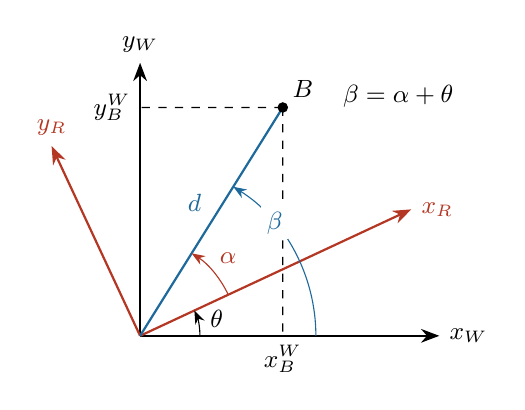
\begin{tikzpicture}[scale=.95]
\coordinate (B) at (58:3.6);
\draw[axis] (0,0)--(4,0) node[right] {$x_W$};
\draw[axis] (0,0)--(0,3.65) node[above] {$y_W$};
\draw[axis,robotframe] (0,0)--(25:4) node[right] {$x_R$};
\draw[axis,robotframe] (0,0)--(115:2.8) node[above] {$y_R$};
\draw[thick,sensorframe] (0,0)--(B) node[midway,above left] {$d$};
\fill (B) circle (2pt) node[above right] {$B$};
\draw[projection] (B)--({3.6*cos(58)},0) node[below] {$x_B^W$};
\draw[projection] (B)--(0,{3.6*sin(58)}) node[left] {$y_B^W$};
\draw[-{Stealth}] (.8,0) arc (0:25:.8);
\node at (12.5:1.05) {$\theta$};
\draw[-{Stealth},robotframe] (25:1.3) arc (25:58:1.3);
\node[robotframe] at (41.5:1.57) {$\alpha$};
\draw[-{Stealth},sensorframe] (2.35,0) arc (0:58:2.35);
\node[sensorframe,fill=white,inner sep=2pt] at (40:2.35) {$\beta$};
\node at (3.45,3.2) {$\beta=\alpha+\theta$};
\end{tikzpicture}

\caption{The same position vector has angle $\alpha$ in $R$ and angle
$\beta=\alpha+\theta$ in $W$. Its length $d$ is independent of the frame.}
\label{fig:l02-angles}
\end{figure}

Expanding the angle sums gives
\begin{align*}
 x_B^W&=d\cos(\alpha+\theta)
 =d\cos\alpha\cos\theta-d\sin\alpha\sin\theta\\
 &=\cos\theta\,x_B^R-\sin\theta\,y_B^R,\\
 y_B^W&=d\sin(\alpha+\theta)
 =d\cos\alpha\sin\theta+d\sin\alpha\cos\theta\\
 &=\sin\theta\,x_B^R+\cos\theta\,y_B^R.
\end{align*}
These are precisely the entries of~\eqref{eq:l02-coordinate-map}. The matrix
formula also applies at $B=O$, where both coordinate vectors are zero and a
direction angle is unnecessary.

\subsection{Worked example: a thirty-degree orientation}
Suppose
\[
 B^R=\begin{bmatrix}0.8\\0.5\end{bmatrix},\qquad \theta=\frac{\pi}{6}.
\]
Then
\begin{align}
 B^W
 &=\begin{bmatrix}\sqrt3/2&-1/2\\1/2&\sqrt3/2\end{bmatrix}
   \begin{bmatrix}0.8\\0.5\end{bmatrix}\\
 &=\begin{bmatrix}0.4\sqrt3-0.25\\0.4+0.25\sqrt3\end{bmatrix}
 \approx\begin{bmatrix}0.4428\\0.8330\end{bmatrix}.
 \label{eq:l02-example}
\end{align}
The coordinates change, but the point's distance from the common origin does
not. Indeed, orthogonality implies
\[
 (B^W)\trans B^W=(B^R)\trans(R_R^W)\trans R_R^W B^R
 =(B^R)\trans B^R=0.8^2+0.5^2=0.89.
\]
This is a change of coordinate description of a fixed point, rather than a
physical motion of that point.

\section{Reversing a coordinate transformation}
To recover robot coordinates from world coordinates, multiply
Equation~\eqref{eq:l02-coordinate-map} on the left by the inverse:
\[
 (R_R^W)^{-1}B^W=(R_R^W)^{-1}R_R^W B^R=B^R.
\]
Using orthogonality,
\begin{equation}
 \boxed{B^R=(R_R^W)\trans B^W=R_W^R B^W,\qquad
 R_W^R=(R_R^W)\trans.}
\end{equation}
Reversing the frame relation exchanges the frame indices and negates the
relative angle. If $R(\theta)$ denotes the matrix in
Equation~\eqref{eq:l02-rotation}, then $R(\theta)\trans=R(-\theta)$.
For arbitrary frames $A$ and $F$, the same rule reads
\begin{equation}
 R_F^A=(R_A^F)\trans.
 \label{eq:l02-swap}
\end{equation}
For example, applying the transpose to the exact vector in
Equation~\eqref{eq:l02-example} recovers $[0.8\;0.5]\trans$.

\section{Composing rotations through several frames}
A measurement may begin in a sensor frame $S$, pass through a robot frame $R$,
and finally be expressed in $W$. Assume again that all origins coincide.
Let the orientation of $R$ relative to $W$ be $\theta$, and the orientation
of $S$ relative to $R$ be $\varphi$.

\begin{figure}[htbp]
\centering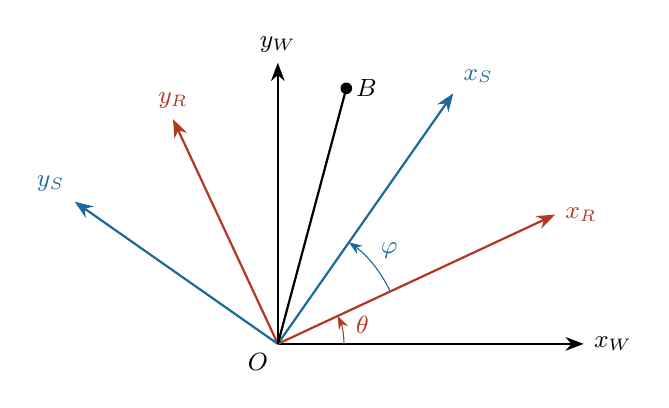
\begin{tikzpicture}[scale=1.05]
\draw[axis] (0,0)--(3.7,0) node[right] {$x_W$};
\draw[axis] (0,0)--(0,3.4) node[above] {$y_W$};
\draw[axis,robotframe] (0,0)--(25:3.7) node[right] {$x_R$};
\draw[axis,robotframe] (0,0)--(115:3) node[above] {$y_R$};
\draw[axis,sensorframe] (0,0)--(55:3.7) node[above right] {$x_S$};
\draw[axis,sensorframe] (0,0)--(145:3) node[above left] {$y_S$};
\draw[-{Stealth},robotframe] (.8,0) arc (0:25:.8);
\node[robotframe] at (12.5:1.05) {$\theta$};
\draw[-{Stealth},sensorframe] (25:1.5) arc (25:55:1.5);
\node[sensorframe] at (40:1.76) {$\varphi$};
\draw[thick] (0,0)--(75:3.2);
\fill (75:3.2) circle (2pt) node[right] {$B$};
\node[below left] at (0,0) {$O$};
\end{tikzpicture}

\caption{Three frames with a common origin. The sensor frame (blue) is rotated
by $\varphi$ relative to the robot frame (red), which is rotated by $\theta$
relative to the world frame (black).}
\label{fig:l02-composition}
\end{figure}

The two successive coordinate transformations are
\[
 B^R=R_S^R B^S,\qquad B^W=R_R^W B^R.
\]
Substitution gives
\begin{equation}
 B^W=R_R^W R_S^R B^S,\qquad
 \boxed{R_S^W=R_R^W R_S^R.}
 \label{eq:l02-chain}
\end{equation}
The rightmost matrix acts first. Its output is expressed in $R$, precisely the
frame expected by the matrix to its left. In two dimensions,
\[
 R_R^W=R(\theta),\qquad R_S^R=R(\varphi),\qquad
 R_S^W=R(\theta+\varphi),
\]
as can be verified with the sine and cosine addition identities.

\subsection{Reading the frame indices}
The general composition rule is
\begin{equation}
 R_C^A=R_B^A R_C^B.
\end{equation}
The subscript of the left factor matches the superscript of the next factor.
The remaining indices identify the overall output and input frames. This is
a rule about the meanings of the maps, not ordinary cancellation of numbers.

For example,
\begin{equation}
 R_2^3 R_4^2 R_5^4 R_1^5=R_1^3.
 \label{eq:l02-long-chain}
\end{equation}
Reading from right to left, the coordinates pass through frames
$1\to5\to4\to2\to3$. By contrast, in the written product $R_2^3 R_3^4$,
the inner frame labels $2$ and $4$ do not match. Its factors cannot be composed
as that sequence of coordinate maps merely by cancelling the repeated $3$.

Planar rotation matrices happen to commute numerically:
$R(\theta)R(\varphi)=R(\varphi)R(\theta)$. This special property does not
change the input and output frame labels of an individual map. Keeping the
frame chain explicit also prepares the notation for three-dimensional
rotations, where commutativity does not hold in general.

\subsection{Simplifying chains containing transposes}
First apply the transpose rules, then inspect the frame chain. Consider
\[
 R_2^3 (R_2^4)\trans (R_5^1 R_4^5)\trans.
\]
Transposing the last product reverses its factor order, so
\begin{align*}
 R_2^3 (R_2^4)\trans (R_5^1 R_4^5)\trans
 &=R_2^3 R_4^2 (R_4^5)\trans (R_5^1)\trans\\
 &=R_2^3 R_4^2 R_5^4 R_1^5\\
 &=R_1^3.
\end{align*}
Two different operations are involved: a transpose exchanges the frame indices
of one rotation matrix, and transposing a product reverses the order of its
factors. Both are necessary to obtain a consistent chain.

\section{The limit of a rotation-only model}
The formula $B^W=R_R^W B^R$ describes point coordinates when the origins
coincide. In a general robot configuration, the origin $O_R$ is displaced from
$O_W$, as in Figure~\ref{fig:l02-translation}. A rotation matrix describes the
relative orientation, but contains no information about this displacement.

\begin{figure}[htbp]
\centering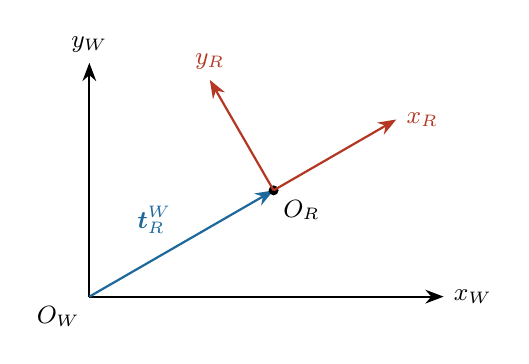
\begin{tikzpicture}[scale=.9]
\draw[axis] (0,0)--(5,0) node[right] {$x_W$};
\draw[axis] (0,0)--(0,3.3) node[above] {$y_W$};
\node[below left] at (0,0) {$O_W$};
\draw[axis,sensorframe] (0,0)--(2.6,1.5) node[midway,above left] {$\boldsymbol{t}_R^W$};
\begin{scope}[shift={(2.6,1.5)}]
\fill (0,0) circle (2pt) node[below right] {$O_R$};
\draw[axis,robotframe] (0,0)--(30:2) node[right] {$x_R$};
\draw[axis,robotframe] (0,0)--(120:1.8) node[above] {$y_R$};
\end{scope}
\end{tikzpicture}

\caption{Different origins introduce a translation $\boldsymbol{t}_R^W$.
Orientation alone cannot determine the world coordinates of a point measured
relative to $O_R$.}
\label{fig:l02-translation}
\end{figure}

To see the limitation, take the point $B=O_R$. Its robot coordinates are zero,
so $R_R^W B^R=0$ for every rotation matrix. Its world coordinates, however,
are the nonzero displacement of $O_R$ from $O_W$. A complete point-coordinate
transformation must therefore include translation as well as rotation.
The rotation rules remain applicable to direction vectors, which do not depend
on the choice of origin. Distinguishing point positions from directions is
essential when extending the model.

\section{Key identities}
\begin{center}
\begin{tabular}{ll}
\toprule
Operation & Identity \\
\midrule
Planar rotation & $R(\theta)=\begin{bmatrix}\cos\theta&-\sin\theta\\\sin\theta&\cos\theta\end{bmatrix}$ \\[12pt]
Point coordinates, common origin & $B^W=R_R^W B^R$ \\
Reverse transformation & $R_W^R=(R_R^W)\trans=R(-\theta)$ \\
Composition & $R_S^W=R_R^W R_S^R$ \\
Planar angle composition & $R(\theta)R(\varphi)=R(\theta+\varphi)$ \\
\bottomrule
\end{tabular}
\end{center}

\clearpage
\section{Additional exercises}
Use column vectors, show your calculations, and label the input and output
frames. Unless stated otherwise, all frames share an origin.
\begin{enumerate}
\item \textbf{Sketching frames and coordinates.}
Draw world axes $x_W,y_W$ and robot axes rotated counterclockwise by $\pi/2$.
A point has $B^R=[2\;1]\trans$. Locate it on your sketch, compute $B^W$,
and check that your answer agrees with its position relative to the world axes.

\item \textbf{Constructing a rotation matrix.}
The robot frame is rotated by $-\pi/4$ relative to the world frame. Write
$[\boldsymbol{x}_R]^W$ and $[\boldsymbol{y}_R]^W$, and use them to construct
$R_R^W$. Verify $(R_R^W)\trans R_R^W=I_2$ and $\det(R_R^W)=1$.

\item \textbf{Forward and reverse transformations.}
Let $\theta_R^W=\pi/6$ and $B^R=[1\;2]\trans$. Find $B^W$ in exact form.
Construct $R_W^R$ and use it to recover $B^R$. Verify that the squared distance
from the common origin is the same in both coordinate descriptions.

\item \textbf{From a sensor to the world.}
Suppose $\theta_R^W=\pi/6$, $\theta_S^R=\pi/3$, and
$B^S=[2\;-1]\trans$. Compute $R_S^W$ and $B^W$. Check your result by first
finding $B^R$ and then transforming it to $W$. What is the orientation of $S$
relative to $W$?

\item \textbf{Frame chains and transposes.}
Simplify the first two expressions to a single rotation matrix. For the third,
explain why the written frame chain is inconsistent, even though the numerical
matrix dimensions permit multiplication:
\[
 R_B^A R_C^B R_D^C,\qquad
 (R_A^B)\trans (R_C^D R_B^C)\trans,\qquad
 R_B^A R_D^C.
\]
Assume distinct letters denote distinct frames. State the input and output
frames of each valid chain.

\item \textbf{Why an origin matters.}
The robot axes are parallel to the world axes, but the robot origin has world
coordinates $[3\;1]\trans$. A point has robot coordinates $[2\;0]\trans$.
Use a sketch to find its world coordinates. What would the rotation-only
formula predict, and what information would it omit?

\item \textbf{Length preservation.}
Let $v^W=R_R^W v^R$ be two coordinate descriptions of a direction vector.
Using orthogonality, show that $(v^W)\trans v^W=(v^R)\trans v^R$.
Explain geometrically why a change of reference frame cannot change the
length of the vector.
\end{enumerate}

\chapter{Planar rigid transformations and homogeneous coordinates}
\label{chap:lecture03}

Rotation describes the relative orientation of two frames, but a mobile robot
also changes position. Its origin generally differs from the origin of the
world map. A sensor mounted on the robot may have yet another origin and
orientation. Relating point coordinates between these frames requires both
rotation and translation.

This chapter extends the rotation model of Chapter~\ref{chap:lecture02} to
planar rigid transformations. The geometric construction leads first to an
affine coordinate relationship, then to a homogeneous matrix representation
that combines rotation and translation in a single multiplication. The same
representation makes composition and inversion systematic.

\section{Rotation and translation between two frames}
Let $O_W$ and $O_R$ be the origins of world frame $W$ and robot frame $R$.
Define
\[
 p_R^W=\begin{bmatrix}p_{Rx}^W\\p_{Ry}^W\end{bmatrix}
\]
as the position of $O_R$ relative to $O_W$, expressed in world coordinates.
The rotation matrix $R_R^W$ describes the orientation of $R$ relative to $W$.
Together, $p_R^W$ and $R_R^W$ specify the robot frame's planar pose.

For a point $B$, the geometric displacement vectors obey
\begin{equation}
 \overrightarrow{O_WB}=\overrightarrow{O_WO_R}+\overrightarrow{O_RB}.
 \label{eq:l03-vector-sum}
\end{equation}
This triangle relation is independent of coordinates. To turn it into a
numerical calculation, however, every vector being added must be expressed
in the same frame.

\begin{figure}[htbp]
\centering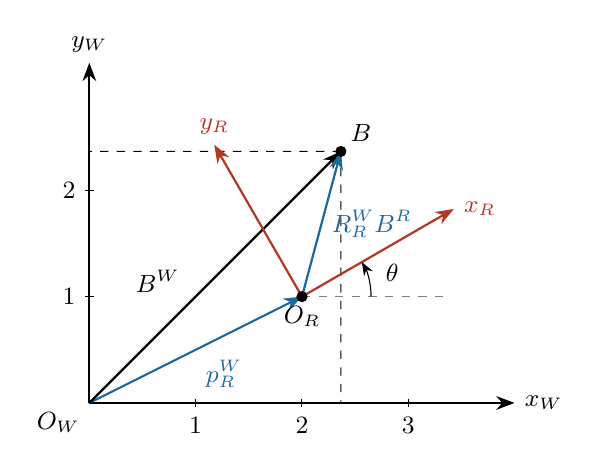
\begin{tikzpicture}[scale=1.35]
\coordinate (O) at (0,0);
\coordinate (R) at (2,1);
\coordinate (B) at (2.366,2.366);
\draw[axis] (O)--(4,0) node[right] {$x_W$};
\draw[axis] (O)--(0,3.2) node[above] {$y_W$};
\foreach \x in {1,2,3} \draw (\x,.04)--(\x,-.04) node[below] {$\x$};
\foreach \y in {1,2} \draw (.04,\y)--(-.04,\y) node[left] {$\y$};
\draw[projection] (B)--(2.366,0);
\draw[projection] (B)--(0,2.366);
\draw[axis,sensorframe] (O)--(R) node[midway,below right] {$p_R^W$};
\draw[axis,thick] (O)--(B) node[pos=.4,above left] {$B^W$};
\draw[axis,sensorframe] (R)--(B) node[midway,right] {$R_R^W B^R$};
\begin{scope}[shift={(R)}]
\draw[axis,robotframe] (0,0)--(30:1.65) node[right] {$x_R$};
\draw[axis,robotframe] (0,0)--(120:1.65) node[above] {$y_R$};
\draw[projection,gray] (0,0)--(1.4,0);
\draw[-{Stealth}] (.65,0) arc (0:30:.65);
\node at (15:.88) {$\theta$};
\end{scope}
\fill (R) circle (1.5pt) node[below] {$O_R$};
\fill (B) circle (1.5pt) node[above right] {$B$};
\node[below left] at (O) {$O_W$};
\end{tikzpicture}

\caption{The displacement to $B$ is the sum of the displacement to the robot
origin and the displacement from that origin to $B$. All three arrow labels
give components in $W$. The geometry uses $p_R^W=[2\;1]\trans$,
$\theta=\pi/6$, and $B^R=[1\;1]\trans$.}
\label{fig:l03-geometry}
\end{figure}

The column $B^R$ contains the components of $\overrightarrow{O_RB}$ along
the robot axes. The column $p_R^W$ uses the world axes. Adding these columns
directly would combine components measured along different directions.
First rotate $B^R$ into world-aligned components; then add the translation:
\begin{equation}
 \boxed{B^W=p_R^W+R_R^W B^R.}
 \label{eq:l03-affine}
\end{equation}
Here $R_R^W B^R$ describes the displacement from $O_R$ to $B$ using world
directions. It is not, by itself, the position of $B$ relative to $O_W$.

\subsection{An intermediate frame makes the geometry explicit}
Introduce a frame $A$ with origin $O_A=O_R$ and axes parallel to those of $W$.
Frames $R$ and $A$ differ only by rotation, so the previous chapter gives
\[
 B^A=R_R^A B^R.
\]
Since $A$ and $W$ have the same orientation, $R_R^A=R_R^W$. Moreover, the
components in $A$ use exactly the directions needed for addition to $p_R^W$.
Thus $B^W=p_R^W+B^A$, recovering Equation~\eqref{eq:l03-affine}.

\begin{figure}[htbp]
\centering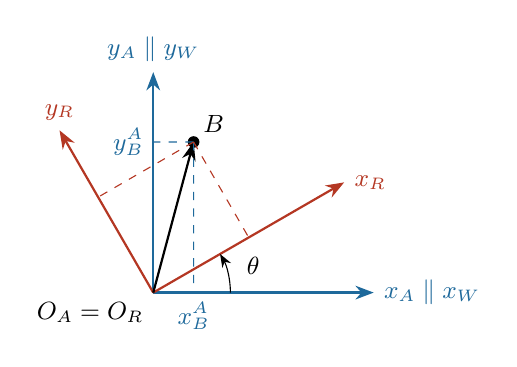
\begin{tikzpicture}[scale=1.4]
\coordinate (B) at (.366,1.366);
\draw[axis,sensorframe] (0,0)--(2,0) node[right] {$x_A\parallel x_W$};
\draw[axis,sensorframe] (0,0)--(0,2) node[above] {$y_A\parallel y_W$};
\draw[axis,robotframe] (0,0)--(30:2) node[right] {$x_R$};
\draw[axis,robotframe] (0,0)--(120:1.7) node[above] {$y_R$};
\draw[axis] (0,0)--(B);
\fill (B) circle (1.5pt) node[above right] {$B$};
\draw[projection,sensorframe] (B)--(.366,0) node[below] {$x_B^A$};
\draw[projection,sensorframe] (B)--(0,1.366) node[left] {$y_B^A$};
\draw[projection,robotframe] (B)--(30:1);
\draw[projection,robotframe] (B)--(120:1);
\draw[-{Stealth}] (.7,0) arc (0:30:.7);
\node at (15:.94) {$\theta$};
\node[below left] at (0,0) {$O_A=O_R$};
\end{tikzpicture}

\caption{The auxiliary frame $A$ shares the robot origin but is aligned with
the world. Rotating from $R$ to $A$ resolves the displacement into components
that can be added to the world position of $O_R$.}
\label{fig:l03-intermediate}
\end{figure}

\subsection{Why the relationship is affine}
A map $f(b)=Rb+p$ is called affine: it consists of a linear map followed by
an offset. With a nonzero translation, it is not a linear map of the original
two coordinates, since $f(0)=p\ne0$. In the present setting $R$ is a rotation,
so the transformation is rigid: it preserves distances between points.
Distances to the coordinate origin need not be preserved when the origin changes.

\subsection{Worked example}
Suppose the given quantities are
\[
 B^R=\begin{bmatrix}1\\1\end{bmatrix}\,\mathrm{m},\qquad
 p_R^W=\begin{bmatrix}2\\1\end{bmatrix}\,\mathrm{m},\qquad
 \theta_R^W=\frac{\pi}{6}.
\]
The rotation matrix is dimensionless. Applying the affine relationship gives
\begin{align}
 B^W
 &=\begin{bmatrix}2\\1\end{bmatrix}
 +\begin{bmatrix}\sqrt3/2&-1/2\\1/2&\sqrt3/2\end{bmatrix}
 \begin{bmatrix}1\\1\end{bmatrix}\\
 &=\begin{bmatrix}(3+\sqrt3)/2\\(3+\sqrt3)/2\end{bmatrix}
 \approx\begin{bmatrix}2.3660\\2.3660\end{bmatrix}\,\mathrm{m}.
 \label{eq:l03-example}
\end{align}
The coordinate arithmetic uses metres throughout. The result agrees with
Figure~\ref{fig:l03-geometry}: the point lies above and slightly to the right
of the robot origin. Keeping the exact expressions until the final step avoids
rounding errors when reversing the calculation.

\section{Reversing the affine relationship}
Suppose $B^W$ is known and $B^R$ is required. Subtract the world-coordinate
translation before applying the inverse rotation:
\begin{align}
 B^W-p_R^W&=R_R^W B^R,\\
 \boxed{B^R=(R_R^W)\trans\bigl(B^W-p_R^W\bigr).}
 \label{eq:l03-affine-inverse}
\end{align}
The difference in parentheses is expressed in $W$; the transpose maps it to
$R$. The parentheses matter: the rotation acts on both terms, not just on $B^W$.
Equivalently,
\begin{equation}
 B^R=-(R_R^W)\trans p_R^W+(R_R^W)\trans B^W.
 \label{eq:l03-inverse-expanded}
\end{equation}
This has the same affine structure as the forward relationship, with
\begin{equation}
 R_W^R=(R_R^W)\trans,\qquad p_W^R=-(R_R^W)\trans p_R^W.
 \label{eq:l03-reverse-pose}
\end{equation}
The reversed translation is not generally just $-p_R^W$: it must also be
expressed along the axes of the reverse transformation's output frame.

For the exact coordinates in Equation~\eqref{eq:l03-example},
\[
 B^W-p_R^W=\begin{bmatrix}(\sqrt3-1)/2\\(1+\sqrt3)/2\end{bmatrix}\,\mathrm{m}.
\]
Multiplying by
$\begin{bmatrix}\sqrt3/2&1/2\\-1/2&\sqrt3/2\end{bmatrix}$
recovers $B^R=[1\;1]\trans\,\mathrm{m}$. If the rounded value
$[2.37\;2.37]\trans$ is used instead, the recovered result is approximately
$[1.0054\;1.0015]\trans\,\mathrm{m}$, rather than exactly $[1\;1]\trans$.

\section{Composing transformations through a sensor frame}
A sensor frame $S$ may be displaced and rotated relative to the robot frame.
Given the sensor's pose in $R$ and the robot's pose in $W$, the two coordinate
relationships are
\[
 B^R=p_S^R+R_S^R B^S,\qquad B^W=p_R^W+R_R^W B^R.
\]
Substitution yields
\begin{align}
 B^W&=p_R^W+R_R^W\bigl(p_S^R+R_S^R B^S\bigr)\\
 &=\underbrace{p_R^W+R_R^W p_S^R}_{p_S^W}
 +\underbrace{R_R^W R_S^R}_{R_S^W}B^S.
 \label{eq:l03-composition-expanded}
\end{align}
The overall rotation and translation are therefore
\begin{equation}
 \boxed{R_S^W=R_R^W R_S^R,\qquad
 p_S^W=p_R^W+R_R^W p_S^R.}
\end{equation}
The sensor translation must be rotated into $W$ before it can be added to
the robot translation. Frame labels explain why the expression is valid and
why simply adding $p_R^W+p_S^R$ would be incorrect in general.

\begin{figure}[htbp]
\centering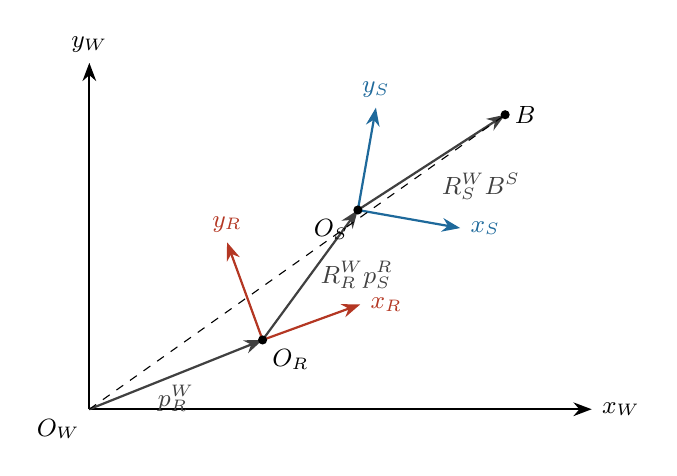
\begin{tikzpicture}[scale=1.1]
\coordinate (R) at (2,.8);
\coordinate (S) at (3.1,2.3);
\coordinate (B) at (4.8,3.4);
\draw[axis] (0,0)--(5.8,0) node[right] {$x_W$};
\draw[axis] (0,0)--(0,4) node[above] {$y_W$};
\node[below left] at (0,0) {$O_W$};
\begin{scope}[shift={(R)}]
\draw[axis,robotframe] (0,0)--(20:1.2) node[right] {$x_R$};
\draw[axis,robotframe] (0,0)--(110:1.2) node[above] {$y_R$};
\end{scope}
\begin{scope}[shift={(S)}]
\draw[axis,sensorframe] (0,0)--(-10:1.2) node[right] {$x_S$};
\draw[axis,sensorframe] (0,0)--(80:1.2) node[above] {$y_S$};
\end{scope}
\draw[axis,black!75] (0,0)--(R) node[midway,below] {$p_R^W$};
\draw[axis,black!75] (R)--(S) node[midway,right] {$R_R^W p_S^R$};
\draw[axis,black!75] (S)--(B) node[midway,below right] {$R_S^W B^S$};
\draw[projection] (0,0)--(B);
\fill (B) circle (1.5pt) node[right] {$B$};
\fill (R) circle (1.5pt) node[below right] {$O_R$};
\fill (S) circle (1.5pt) node[below left] {$O_S$};
\end{tikzpicture}

\caption{A world--robot--sensor chain with distinct origins. Each displacement
along the path to $B$ is labeled in world components so that the arrows can be
added numerically. The dashed line is the direct displacement to $B$.}
\label{fig:l03-composition}
\end{figure}

Repeated substitution works for any number of frames, but each additional
frame introduces another translation term. A representation that absorbs
these additions into matrix multiplication makes longer chains easier to manage.

\section{Homogeneous coordinates and transformation matrices}
\subsection{Adding one coordinate}
For a point with coordinates $B^R$, define its homogeneous representation by
appending a dimensionless one:
\begin{equation}
 \widetilde B^R=\begin{bmatrix}B^R\\1\end{bmatrix}
 =\begin{bmatrix}x_B^R\\y_B^R\\1\end{bmatrix}.
\end{equation}
The additional coordinate is bookkeeping for translation, not a third spatial
coordinate. Define the planar homogeneous transformation matrix as
\begin{equation}
 \boxed{H_R^W=\begin{bmatrix}R_R^W&p_R^W\\0_{1\times2}&1\end{bmatrix}.}
 \label{eq:l03-H}
\end{equation}
Its blocks have dimensions $2\times2$, $2\times1$, $1\times2$, and $1\times1$,
respectively. Written entry by entry, it is
\[
 H_R^W=\begin{bmatrix}
 \cos\theta&-\sin\theta&p_{Rx}^W\\
 \sin\theta&\cos\theta&p_{Ry}^W\\
 0&0&1
 \end{bmatrix}.
\]
The upper-left block contains dimensionless rotation coefficients; the first
two entries of the last column carry the chosen length unit. Block divisions
are visual aids, not extra mathematical operations.

\subsection{One product performs the full transformation}
Block multiplication gives
\begin{equation}
 H_R^W\widetilde B^R
 =\begin{bmatrix}R_R^W&p_R^W\\0_{1\times2}&1\end{bmatrix}
 \begin{bmatrix}B^R\\1\end{bmatrix}
 =\begin{bmatrix}R_R^W B^R+p_R^W\\1\end{bmatrix}
 =\widetilde B^W.
\end{equation}
Thus the affine transformation becomes a single matrix multiplication:
\begin{equation}
 \boxed{\widetilde B^W=H_R^W\widetilde B^R.}
 \label{eq:l03-homogeneous-map}
\end{equation}
The first two output entries are the desired point coordinates. For the
normalized point representation used here, the last entry remains one.
The fixed bottom row $[0\;0\;1]$ is what preserves this property.

For the running example, using metres for the position entries,
\[
 \begin{bmatrix}\sqrt3/2&-1/2&2\\1/2&\sqrt3/2&1\\0&0&1\end{bmatrix}
 \begin{bmatrix}1\\1\\1\end{bmatrix}
 =\begin{bmatrix}(3+\sqrt3)/2\\(3+\sqrt3)/2\\1\end{bmatrix}
 \approx\begin{bmatrix}2.3660\\2.3660\\1\end{bmatrix}.
\]
The physical point coordinates are the first two entries in metres; the final
one has no length unit.

\section{Composition by matrix multiplication}
Using homogeneous coordinates for the sensor chain,
\[
 \widetilde B^R=H_S^R\widetilde B^S,\qquad
 \widetilde B^W=H_R^W\widetilde B^R.
\]
Combining the two maps gives
\begin{equation}
 \boxed{H_S^W=H_R^W H_S^R,\qquad
 \widetilde B^W=H_R^W H_S^R\widetilde B^S.}
\end{equation}
Multiplying the blocks verifies that this contains both composition rules:
\begin{align}
 H_R^W H_S^R
 &=\begin{bmatrix}R_R^W&p_R^W\\0&1\end{bmatrix}
   \begin{bmatrix}R_S^R&p_S^R\\0&1\end{bmatrix}\\
 &=\begin{bmatrix}
 R_R^W R_S^R&p_R^W+R_R^W p_S^R\\0&1
 \end{bmatrix}=H_S^W.
\end{align}
Here each $0$ in the bottom-left block denotes a $1\times2$ zero row.
The product is another homogeneous rigid transformation with bottom row
$[0\;0\;1]$. As before, the rightmost map acts first and adjacent frame
indices must match. For example,
\[
 H_1^2 H_3^1 H_4^3 H_5^4=H_5^2
\]
maps coordinates through $5\to4\to3\to1\to2$.

Unlike pure planar rotations, planar transformations with translation do not
generally commute. The term $R_R^W p_S^R$ shows why: a preceding rotation
changes the direction in which a subsequent local translation acts.

\section{Inverting a homogeneous transformation}
\subsection{Why the transpose is insufficient}
Expanding the determinant along the bottom row gives
\[
 \det(H_R^W)=\det(R_R^W)=1.
\]
Every matrix of this rigid-transformation form is therefore invertible.
However, it is generally not orthogonal. If its translation is nonzero, its
transpose has bottom row $[(p_R^W)\trans\;1]$ rather than $[0\;0\;1]$.
Consequently, transposing the full matrix does not produce its inverse.
When the translation is zero, the full matrix is orthogonal and the transpose
does coincide with the inverse.

\subsection{Deriving the inverse from the affine relationship}
Equation~\eqref{eq:l03-inverse-expanded} already identifies the reverse
rotation and translation. Place these in their corresponding blocks:
\begin{equation}
 \boxed{H_W^R=(H_R^W)^{-1}
 =\begin{bmatrix}
 (R_R^W)\trans&-(R_R^W)\trans p_R^W\\0_{1\times2}&1
 \end{bmatrix}.}
 \label{eq:l03-H-inverse}
\end{equation}
This gives $\widetilde B^R=H_W^R\widetilde B^W$ without a general-purpose
$3\times3$ inversion. Transpose the rotation block, compute the rotated
negative translation, and retain the bottom row.

\begin{figure}[htbp]
\centering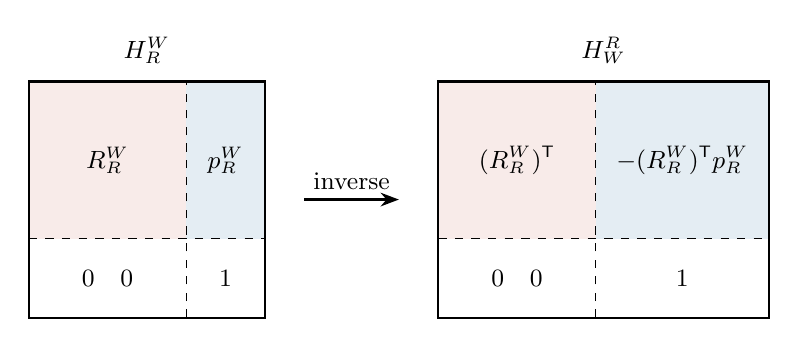
\begin{tikzpicture}
\fill[robotframe!10] (0,1) rectangle (2,3);
\fill[sensorframe!12] (2,1) rectangle (3,3);
\draw[thick] (0,0) rectangle (3,3);
\draw[dashed] (2,0)--(2,3) (0,1)--(3,1);
\node at (1,2) {$R_R^W$};
\node at (2.5,2) {$p_R^W$};
\node at (1,.5) {$0\quad0$};
\node at (2.5,.5) {$1$};
\node[above] at (1.5,3.1) {$H_R^W$};
\draw[axis] (3.5,1.5)--(4.7,1.5) node[midway,above] {inverse};
\begin{scope}[shift={(5.2,0)}]
\fill[robotframe!10] (0,1) rectangle (2,3);
\fill[sensorframe!12] (2,1) rectangle (4.2,3);
\draw[thick] (0,0) rectangle (4.2,3);
\draw[dashed] (2,0)--(2,3) (0,1)--(4.2,1);
\node at (1,2) {$(R_R^W)\trans$};
\node at (3.1,2) {$-(R_R^W)\trans p_R^W$};
\node at (1,.5) {$0\quad0$};
\node at (3.1,.5) {$1$};
\node[above] at (2.1,3.1) {$H_W^R$};
\end{scope}
\end{tikzpicture}

\caption{Block structure of a transform and its inverse. Red blocks contain
rotation; blue blocks contain translation. The inverse translation must be
rotated as well as negated. Block widths are schematic.}
\label{fig:l03-blocks}
\end{figure}

For a compact verification, write $R=R_R^W$ and $p=p_R^W$. Then
\[
 \begin{bmatrix}R&p\\0&1\end{bmatrix}
 \begin{bmatrix}R\trans&-R\trans p\\0&1\end{bmatrix}
 =\begin{bmatrix}RR\trans&-RR\trans p+p\\0&1\end{bmatrix}=I_3.
\]
The reverse product also equals $I_3$, since its translation block is
$R\trans p-R\trans p=0$.

\subsection{Worked inverse}
For $p_R^W=[2\;1]\trans\,\mathrm{m}$ and $\theta_R^W=\pi/6$,
\begin{align*}
 -(R_R^W)\trans p_R^W
 &=-\begin{bmatrix}\sqrt3/2&1/2\\-1/2&\sqrt3/2\end{bmatrix}
 \begin{bmatrix}2\\1\end{bmatrix}\\
 &=\begin{bmatrix}-\sqrt3-1/2\\1-\sqrt3/2\end{bmatrix}
 \approx\begin{bmatrix}-2.2321\\0.1340\end{bmatrix}\,\mathrm{m}.
\end{align*}
Hence, with translation entries in metres,
\begin{equation}
 H_W^R=\begin{bmatrix}
 \sqrt3/2&1/2&-\sqrt3-1/2\\
 -1/2&\sqrt3/2&1-\sqrt3/2\\
 0&0&1
 \end{bmatrix}.
\end{equation}
Its last column locates the world origin in robot coordinates. Its upper-left
block describes the world axes in the robot frame. These meanings provide
geometric checks on the inverse, in addition to verifying the matrix product.

\section{Key identities}
\begin{center}
\renewcommand{\arraystretch}{1.35}
\begin{tabular}{ll}
\toprule
Operation & Identity \\
\midrule
Forward point transformation & $B^W=p_R^W+R_R^W B^R$ \\
Reverse point transformation & $B^R=(R_R^W)\trans(B^W-p_R^W)$ \\
Homogeneous point transformation & $\widetilde B^W=H_R^W\widetilde B^R$ \\
Composition & $H_S^W=H_R^W H_S^R$ \\
Reverse rotation & $R_W^R=(R_R^W)\trans$ \\
Reverse translation & $p_W^R=-(R_R^W)\trans p_R^W$ \\
\bottomrule
\end{tabular}
\end{center}
Always specify the frame of a translation, express displacements in a common
frame before adding them, and distinguish the inverse of a rotation matrix
from the inverse of a full homogeneous transformation.

\clearpage
\section{Additional exercises}
Use metres for all position coordinates and counterclockwise-positive angles.
Show your calculations and keep exact values until the final numerical step.
\begin{enumerate}
\item \textbf{A translated and rotated robot.}
Let $p_R^W=[3\;1]\trans$, $\theta_R^W=\pi/2$, and
$B^R=[2\;-1]\trans$. Sketch the two frames and the point. Compute $B^W$
using the affine relationship and explain why $p_R^W+B^R$ gives a different result.

\item \textbf{Recovering robot coordinates.}
Suppose $p_R^W=[1\;-2]\trans$, $\theta_R^W=-\pi/2$, and
$B^W=[4\;-3]\trans$. Find $B^R$. Substitute it into the forward
relationship to verify your answer. State the frame of every vector being added.

\item \textbf{Building a homogeneous matrix.}
Construct $H_R^W$ for $p_R^W=[2\;0]\trans$ and $\theta_R^W=\pi/4$.
Use it to transform $B^R=[\sqrt2\;0]\trans$. Identify the physical
coordinates in the output and explain the role of its last entry.

\item \textbf{World--robot--sensor composition.}
Let $p_R^W=[2\;1]\trans$, $\theta_R^W=\pi/2$,
$p_S^R=[1\;0]\trans$, and $\theta_S^R=-\pi/2$.
Find $H_S^W=H_R^W H_S^R$ and use it to transform $B^S=[1\;2]\trans$.
Check your result by applying the two affine transformations separately.

\item \textbf{Inversion without a general matrix inverse.}
For
\[
 H_R^W=\begin{bmatrix}0&-1&2\\1&0&3\\0&0&1\end{bmatrix},
\]
compute $H_W^R$ using its rotation and translation blocks. Verify
$H_W^R H_R^W=I_3$. Compare your result with $(H_R^W)\trans$ and identify
why the transpose fails.

\item \textbf{Order of operations.}
Consider the two maps, expressed using a fixed coordinate system,
\[
 T=\begin{bmatrix}1&0&1\\0&1&0\\0&0&1\end{bmatrix},\qquad
 Q=\begin{bmatrix}0&-1&0\\1&0&0\\0&0&1\end{bmatrix}.
\]
Compute $QT$ and $TQ$ and apply each to $[0\;0\;1]\trans$.
Explain geometrically why rotating after translating differs from translating
after rotating.

\item \textbf{Distances between points.}
Two points obey $B^W=p+RB^R$ and $C^W=p+RC^R$, with $R$ orthogonal.
Show that $B^W-C^W=R(B^R-C^R)$ and use this to prove that their distance
is preserved. Why need the distance of a single point from its coordinate
origin not be preserved?
\end{enumerate}

\chapter{Three-dimensional rotations and orientation representations}
\label{chap:lecture04}

A robot that moves outside a plane requires a spatial description of
orientation. One angle no longer suffices: a body can turn about three
independent directions. The construction of a rotation matrix remains the
same, however. Its columns are the unit axes of one frame expressed in another.
In three dimensions, these columns have three components, giving a $3\times3$
matrix.

This chapter constructs rotations about individual axes, combines them into
a yaw--pitch--roll sequence, recovers those angles from a rotation matrix,
and introduces unit quaternions as a practical orientation representation.
All frames used for point-coordinate transformations here share an origin;
translation is set aside so that the orientation conventions can be developed
explicitly.

\section{Spatial frames and rotation matrices}
Let $W$ be a right-handed world frame and $R$ a right-handed robot frame.
Each has three mutually perpendicular unit axes. Write the robot's axes in
world components as $[\boldsymbol{x}_R]^W$, $[\boldsymbol{y}_R]^W$, and
$[\boldsymbol{z}_R]^W$. Then
\begin{equation}
 R_R^W=\begin{bmatrix}
 [\boldsymbol{x}_R]^W &[\boldsymbol{y}_R]^W &[\boldsymbol{z}_R]^W
 \end{bmatrix}\in\R^{3\times3}.
 \label{eq:l04-columns}
\end{equation}
As in the planar case, the subscript gives the input frame and the superscript
gives the output frame of the coordinate map. For a point $B$ and common origins,
\begin{equation}
 B^W=R_R^W B^R,\qquad
 B^R=\begin{bmatrix}x_B^R\\y_B^R\\z_B^R\end{bmatrix}.
\end{equation}
The same rotation maps the components of a direction vector between frames
regardless of the locations of their origins.

Positive elementary angles follow the right-hand rule: point the right thumb
along the positive rotation axis and curl the fingers in the positive direction.
Viewed from the positive end of that axis toward the origin, the positive
rotation appears counterclockwise. A perspective drawing may distort lengths
and visible angles; it does not change this convention.

\section{Elementary rotations}
An elementary rotation leaves one axis fixed and rotates the perpendicular
plane. The three basic cases are shown in Figure~\ref{fig:l04-elementary}.
Each is constructed by expressing the rotated basis vectors in the original
frame, then placing those vectors in columns.

\begin{figure}[htbp]
\centering% Three exact 3D constructions projected onto the page; lengths in the
% projection are not physical lengths. The red axes are matrix columns.
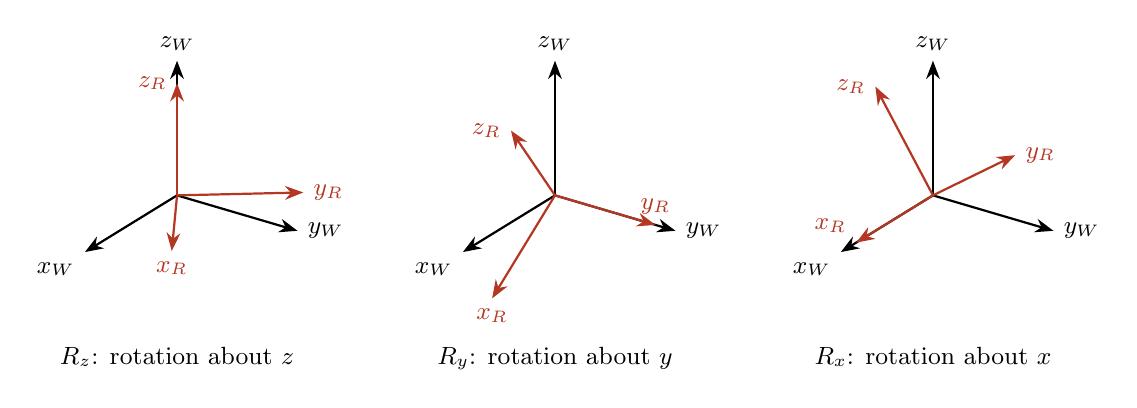
\begin{tikzpicture}[x={(-.65cm,-.4cm)},y={(.85cm,-.25cm)},z={(0cm,.95cm)}]
\foreach \panel/\name in {0/z,4.8/y,9.6/x} {
\begin{scope}[shift={(\panel cm,0cm)}]
\draw[axis] (0,0,0)--(1.8,0,0) node[below left] {$x_W$};
\draw[axis] (0,0,0)--(0,1.8,0) node[right] {$y_W$};
\draw[axis] (0,0,0)--(0,0,1.8) node[above] {$z_W$};
\if\name z
 \draw[axis,robotframe] (0,0,0)--({1.5*cos(35)},{1.5*sin(35)},0) node[below] {$x_R$};
 \draw[axis,robotframe] (0,0,0)--({-1.5*sin(35)},{1.5*cos(35)},0) node[right] {$y_R$};
 \draw[axis,robotframe] (0,0,0)--(0,0,1.5) node[left] {$z_R$};
\fi
\if\name y
 \draw[axis,robotframe] (0,0,0)--({1.5*cos(35)},0,{-1.5*sin(35)}) node[below] {$x_R$};
 \draw[axis,robotframe] (0,0,0)--(0,1.5,0) node[above] {$y_R$};
 \draw[axis,robotframe] (0,0,0)--({1.5*sin(35)},0,{1.5*cos(35)}) node[left] {$z_R$};
\fi
\if\name x
 \draw[axis,robotframe] (0,0,0)--(1.5,0,0) node[above left] {$x_R$};
 \draw[axis,robotframe] (0,0,0)--(0,{1.5*cos(35)},{1.5*sin(35)}) node[right] {$y_R$};
 \draw[axis,robotframe] (0,0,0)--(0,{-1.5*sin(35)},{1.5*cos(35)}) node[left] {$z_R$};
\fi
\node at (0,-1.7,0) {};
\node[anchor=north] at (0cm,-1.8cm) {$R_{\name}$: rotation about $\name$};
\end{scope}
}
\end{tikzpicture}

\caption{Elementary rotations in perspective. Black axes are the world frame;
red axes are the rotated frame. The rotation axis is shared by the two frames.
The three panels are separate constructions, each with a positive angle.}
\label{fig:l04-elementary}
\end{figure}

\subsection{Rotation about the z axis}
Let $\psi$ denote a rotation about $z_W$. The $z$ axis remains unchanged, while
the $x$ and $y$ axes rotate in the $xy$ plane:
\[
 [\boldsymbol{x}_R]^W=\begin{bmatrix}\cos\psi\\\sin\psi\\0\end{bmatrix},\quad
 [\boldsymbol{y}_R]^W=\begin{bmatrix}-\sin\psi\\\cos\psi\\0\end{bmatrix},\quad
 [\boldsymbol{z}_R]^W=\begin{bmatrix}0\\0\\1\end{bmatrix}.
\]
Therefore,
\begin{equation}
 \boxed{R_z(\psi)=\begin{bmatrix}
 \cos\psi&-\sin\psi&0\\\sin\psi&\cos\psi&0\\0&0&1
 \end{bmatrix}.}
 \label{eq:l04-rz}
\end{equation}
The upper-left block is exactly the planar rotation matrix. The last coordinate
is unchanged because the rotation takes place in the plane perpendicular to $z$.

\subsection{Rotation about the y axis}
For a positive angle $\theta$ about $y_W$, the $x$ axis turns toward negative
$z$ and the $z$ axis turns toward positive $x$. The basis columns are
\[
 [\boldsymbol{x}_R]^W=\begin{bmatrix}\cos\theta\\0\\-\sin\theta\end{bmatrix},\quad
 [\boldsymbol{y}_R]^W=\begin{bmatrix}0\\1\\0\end{bmatrix},\quad
 [\boldsymbol{z}_R]^W=\begin{bmatrix}\sin\theta\\0\\\cos\theta\end{bmatrix}.
\]
Thus
\begin{equation}
 \boxed{R_y(\theta)=\begin{bmatrix}
 \cos\theta&0&\sin\theta\\0&1&0\\-\sin\theta&0&\cos\theta
 \end{bmatrix}.}
 \label{eq:l04-ry}
\end{equation}
The signs follow from the right-hand rule. The two-dimensional pattern is
visible in the ordered plane $(z,x)$, where positive rotation carries $z$
toward $x$; using the order $(x,z)$ without accounting for orientation would
reverse the signs.

\subsection{Rotation about the x axis}
For a positive angle $\varphi$ about $x_W$, the $x$ axis is fixed and the
$y$ axis turns toward positive $z$. Hence
\[
 [\boldsymbol{x}_R]^W=\begin{bmatrix}1\\0\\0\end{bmatrix},\quad
 [\boldsymbol{y}_R]^W=\begin{bmatrix}0\\\cos\varphi\\\sin\varphi\end{bmatrix},\quad
 [\boldsymbol{z}_R]^W=\begin{bmatrix}0\\-\sin\varphi\\\cos\varphi\end{bmatrix},
\]
and
\begin{equation}
 \boxed{R_x(\varphi)=\begin{bmatrix}
 1&0&0\\0&\cos\varphi&-\sin\varphi\\0&\sin\varphi&\cos\varphi
 \end{bmatrix}.}
 \label{eq:l04-rx}
\end{equation}

\begin{figure}[htbp]
\centering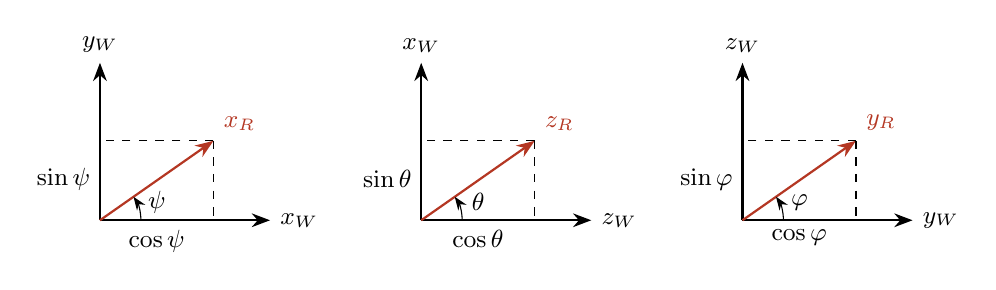
\begin{tikzpicture}[scale=.8]
\foreach \shift/\horizontal/\vertical/\angle/\moving in {
0/x_W/y_W/\psi/x_R,5.1/z_W/x_W/\theta/z_R,10.2/y_W/z_W/\varphi/y_R} {
\begin{scope}[shift={(\shift,0)}]
\draw[axis] (0,0)--(2.7,0) node[right] {$\horizontal$};
\draw[axis] (0,0)--(0,2.5) node[above] {$\vertical$};
\draw[axis,robotframe] (0,0)--(35:2.2) node[above right] {$\moving$};
\draw[projection] (35:2.2)--({2.2*cos(35)},0);
\draw[projection] (35:2.2)--(0,{2.2*sin(35)});
\node[below] at (.9,0) {$\cos\angle$};
\node[left] at (0,.65) {$\sin\angle$};
\draw[-{Stealth}] (.65,0) arc (0:35:.65);
\node at (17.5:.95) {$\angle$};
\end{scope}
}
\end{tikzpicture}

\caption{Plane views of the elementary rotations. From left to right, the
ordered planes are $(x_W,y_W)$, $(z_W,x_W)$, and $(y_W,z_W)$. Each red
vector has unit length; its projections explain the sine and cosine entries.}
\label{fig:l04-planes}
\end{figure}

A quick sign check is to use a quarter-turn: $R_z(\pi/2)$ maps the first
basis vector to the second, $R_y(\pi/2)$ maps the third to the first, and
$R_x(\pi/2)$ maps the second to the third. At zero angle, all three matrices
reduce to $I_3$.

\section{What makes a matrix a valid spatial rotation?}
Write $R=[u\;v\;w]$. Its columns must be unit vectors and mutually
perpendicular:
\begin{equation}
 u\trans u=v\trans v=w\trans w=1,\qquad
 u\trans v=u\trans w=v\trans w=0.
 \label{eq:l04-constraints}
\end{equation}
Together these six scalar constraints give $R\trans R=I_3$. They constrain
the nine matrix entries to three continuous degrees of freedom. To describe
a rotation between right-handed frames, rather than a reflection, one also
requires $\det R=+1$. The determinant condition selects the proper-rotation
component; it does not remove another continuous degree of freedom.

For a valid rotation,
\begin{equation}
 R^{-1}=R\trans,\qquad R_F^A=(R_A^F)\trans.
\end{equation}
Composition still follows the frame chain, $R_C^A=R_B^A R_C^B$, and lengths
are preserved. These are the same structural properties used in two dimensions.

\subsection{An illustrative set of components}
To illustrate how columns are assembled, consider the rough component array
\begin{equation}
 M=\begin{bmatrix}.8&-.3&.4\\.2&.7&.15\\-.1&.2&.7\end{bmatrix}.
 \label{eq:l04-rough}
\end{equation}
Its first column describes a direction with a large positive $x$ component,
a smaller positive $y$ component, and a negative $z$ component. The other
columns can be read in the same way. However, these illustrative numbers do
\emph{not} define a rotation matrix. For example,
\[
 u\trans u=.8^2+.2^2+(-.1)^2=.69\ne1,\qquad
 u\trans v=.8(-.3)+.2(.7)+(-.1)(.2)=-.12\ne0.
\]
Even normalizing each column separately would not make the columns mutually
perpendicular. A valid frame must satisfy all the orthonormality conditions
and the right-handedness condition, not just have plausible-looking components.

\section{Roll, pitch, and yaw as a sequence of rotations}
A general spatial orientation can be represented by a sequence of three
elementary rotations. Many sequences are possible, and the convention must
be specified before interpreting three angle values. Here the convention is
the \emph{intrinsic Z--Y--X sequence}: each successive rotation is about an
axis of the frame obtained after the previous rotation.

Starting from frame $W$, define intermediate frames 1 and 2 and final frame 3:
\begin{enumerate}
 \item Rotate by yaw $\psi$ about $z_W$ to obtain frame 1.
 \item Rotate by pitch $\theta$ about the new axis $y_1$ to obtain frame 2.
 \item Rotate by roll $\varphi$ about the new axis $x_2$ to obtain frame 3.
\end{enumerate}
Although the angles are often listed as roll, pitch, yaw, the construction
above proceeds through yaw, pitch, then roll.

\begin{figure}[htbp]
\centering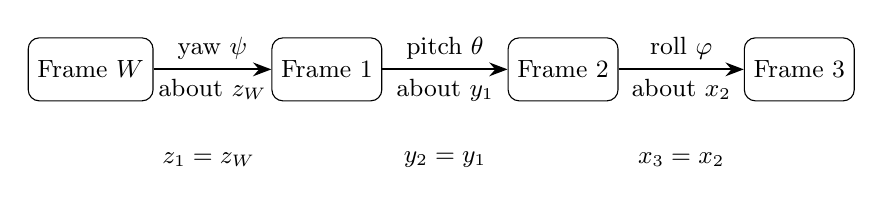
\begin{tikzpicture}
\foreach \x/\frame in {0/W,3/1,6/2,9/3} {
 \node[draw,rounded corners,minimum width=1cm,minimum height=.8cm] (f\frame) at (\x,0) {Frame $\frame$};
}
\draw[axis] (fW)--(f1) node[midway,above] {yaw $\psi$} node[midway,below] {about $z_W$};
\draw[axis] (f1)--(f2) node[midway,above] {pitch $\theta$} node[midway,below] {about $y_1$};
\draw[axis] (f2)--(f3) node[midway,above] {roll $\varphi$} node[midway,below] {about $x_2$};
\node at (1.5,-1.15) {$z_1=z_W$};
\node at (4.5,-1.15) {$y_2=y_1$};
\node at (7.5,-1.15) {$x_3=x_2$};
\end{tikzpicture}

\caption{The intrinsic Z--Y--X construction. The axis used at each stage stays
fixed during that stage. Arrows show the sequence of frame construction;
coordinate maps from frame 3 back to $W$ act in the reverse traversal.}
\label{fig:l04-sequence}
\end{figure}

The elementary frame relationships are
\[
 R_1^W=R_z(\psi),\qquad R_2^1=R_y(\theta),\qquad R_3^2=R_x(\varphi).
\]
Applying the frame-chain rule gives
\begin{equation}
 \boxed{R_3^W=R_1^W R_2^1 R_3^2
 =R_z(\psi)R_y(\theta)R_x(\varphi).}
 \label{eq:l04-rpy}
\end{equation}
This product maps coordinates from frame 3 to $W$. When it multiplies $B^3$,
the rightmost factor acts first: $B^3\to B^2\to B^1\to B^W$. This algebraic
order is consistent with constructing the frames successively about their
moving axes; it should not be confused with three rotations about fixed world
axes in the same chronological order.

\subsection{Order matters in three dimensions}
Unlike planar rotations, rotations about different spatial axes do not
generally commute. With $e_x=[1\;0\;0]\trans$,
\[
 R_z(\pi/2)R_x(\pi/2)e_x=e_y,\qquad
 R_x(\pi/2)R_z(\pi/2)e_x=e_z.
\]
The first product leaves $e_x$ unchanged in its first step, then turns it
toward $e_y$. The second turns it toward $e_y$ first, then toward $e_z$.
Thus changing the factor order generally changes the orientation.

\subsection{Expanded form}
For compactness, write $c_a=\cos a$ and $s_a=\sin a$. Multiplying the three
elementary matrices yields
\begin{equation}
 R=\begin{bmatrix}
 c_\psi c_\theta & c_\psi s_\theta s_\varphi-s_\psi c_\varphi & c_\psi s_\theta c_\varphi+s_\psi s_\varphi\\
 s_\psi c_\theta & s_\psi s_\theta s_\varphi+c_\psi c_\varphi & s_\psi s_\theta c_\varphi-c_\psi s_\varphi\\
 -s_\theta & c_\theta s_\varphi & c_\theta c_\varphi
 \end{bmatrix}.
 \label{eq:l04-expanded}
\end{equation}
The factored form is often easier to evaluate and check. The expanded form is
particularly useful for identifying which entries contain the information
needed to recover the angles.

\section{Worked example}
Let the roll, pitch, and yaw angles be
\[
 \varphi=\frac{\pi}{4},\qquad \theta=\frac{\pi}{3},\qquad \psi=\frac{\pi}{2}.
\]
Then
\begin{align}
 R_3^W
 &=\begin{bmatrix}0&-1&0\\1&0&0\\0&0&1\end{bmatrix}
 \begin{bmatrix}1/2&0&\sqrt3/2\\0&1&0\\-\sqrt3/2&0&1/2\end{bmatrix}
 \begin{bmatrix}1&0&0\\0&\sqrt2/2&-\sqrt2/2\\0&\sqrt2/2&\sqrt2/2\end{bmatrix}\\
 &=\begin{bmatrix}
 0&-\sqrt2/2&\sqrt2/2\\
 1/2&\sqrt6/4&\sqrt6/4\\
 -\sqrt3/2&\sqrt2/4&\sqrt2/4
 \end{bmatrix}.
 \label{eq:l04-example}
\end{align}
For instance, the first column has squared length $1/4+3/4=1$ and has zero
dot product with the second column. More generally, the product of these
three proper rotation matrices is itself a proper rotation matrix.

If $B^3=[1\;0\;0]\trans$, its world coordinates are the first column of
$R_3^W$. To return to frame 3, use $(R_3^W)\trans$. Thus the orientation
representation serves directly as a coordinate transformation.

\section{Recovering roll, pitch, and yaw}
Let a valid rotation matrix be written as
\[
 R=\begin{bmatrix}r_{11}&r_{12}&r_{13}\\r_{21}&r_{22}&r_{23}\\r_{31}&r_{32}&r_{33}\end{bmatrix}.
\]
For the convention in Equation~\eqref{eq:l04-rpy}, choose the principal pitch
range $-\pi/2<\theta<\pi/2$. In this nonsingular range,
\begin{equation}
 \boxed{\begin{aligned}
 \varphi&=\operatorname{atan2}(r_{32},r_{33}),\\
 \theta&=\operatorname{atan2}\!\left(-r_{31},\sqrt{r_{32}^2+r_{33}^2}\right),\\
 \psi&=\operatorname{atan2}(r_{21},r_{11}).
 \end{aligned}}
 \label{eq:l04-extraction}
\end{equation}
The entries in Equation~\eqref{eq:l04-expanded} explain these formulas:
\[
 (r_{32},r_{33})=c_\theta(s_\varphi,c_\varphi),\qquad
 (r_{21},r_{11})=c_\theta(s_\psi,c_\psi).
\]
Since $c_\theta>0$ on the chosen range, each pair has the same direction as
the corresponding sine--cosine pair. Also,
\[
 -r_{31}=s_\theta,\qquad
 \sqrt{r_{32}^2+r_{33}^2}=|c_\theta|=c_\theta.
\]
Applied to Equation~\eqref{eq:l04-example}, the formulas give
\[
 \varphi=\operatorname{atan2}(\sqrt2/4,\sqrt2/4)=\pi/4,
 \quad \theta=\operatorname{atan2}(\sqrt3/2,1/2)=\pi/3,
\]
and $\psi=\operatorname{atan2}(1/2,0)=\pi/2$, recovering the original angles.

\subsection{Why atan2 takes two arguments}
The function $\operatorname{atan2}(y,x)$ returns the angle of the pair $(x,y)$,
using both signs to identify the quadrant. The argument order here is
\emph{vertical component first, horizontal component second}. The numeral 2
is part of the function's name, not a multiplication or exponent.

The ratio $y/x$ alone loses information: $(1,1)$ and $(-1,-1)$ both have ratio
one, but point in opposite directions. Ordinary $\arctan(y/x)$ returns the
same principal angle for both, whereas
\[
 \operatorname{atan2}(1,1)=\pi/4,\qquad
 \operatorname{atan2}(-1,-1)=-3\pi/4.
\]
Unlike division followed by arctangent, $\operatorname{atan2}$ also handles
$x=0$ with $y\ne0$, giving $\pi/2$ or $-\pi/2$.

\begin{figure}[htbp]
\centering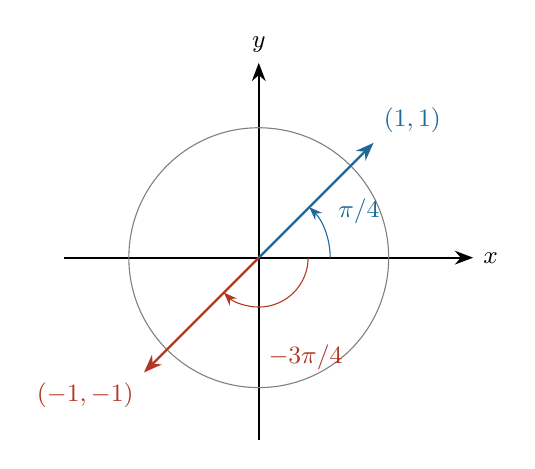
\begin{tikzpicture}[scale=1.65]
\draw[axis] (-1.5,0)--(1.65,0) node[right] {$x$};
\draw[axis] (0,-1.4)--(0,1.5) node[above] {$y$};
\draw[gray] (0,0) circle (1);
\draw[axis,sensorframe] (0,0)--(45:1.25) node[above right] {$(1,1)$};
\draw[axis,robotframe] (0,0)--(225:1.25) node[below left] {$(-1,-1)$};
\draw[-{Stealth},sensorframe] (.55,0) arc (0:45:.55);
\node[sensorframe] at (25:.85) {$\pi/4$};
\draw[-{Stealth},robotframe] (.38,0) arc (0:-135:.38);
\node[robotframe] at (-65:.85) {$-3\pi/4$};
\end{tikzpicture}

\caption{Equal ratios do not imply equal directions. The signs of both
components distinguish the first and third quadrants. The circle indicates
direction only; the two labeled vectors need not have unit length.}
\label{fig:l04-atan2}
\end{figure}

Tangent has period $\pi$, while a full revolution has length $2\pi$.
The principal arctangent takes values in $(-\pi/2,\pi/2)$; a conventional
principal range for $\operatorname{atan2}$ spans $2\pi$, such as $(-\pi,\pi]$.
At the negative horizontal axis, $\pi$ and $-\pi$ represent the same direction;
endpoint handling can vary between implementations. At $(x,y)=(0,0)$ there is
no geometric direction, whatever numerical value a software routine returns.

\subsection{Singular orientations and angle ranges}
The three-angle representation covers all orientations, but is not globally
unique or nonsingular. At $\theta=\pm\pi/2$, the pairs used to extract yaw
and roll both vanish:
\[
 r_{32}=r_{33}=r_{21}=r_{11}=0.
\]
Consequently, Equation~\eqref{eq:l04-extraction} cannot determine yaw and roll
separately. At $\theta=\pi/2$, for example, the matrix depends on their
difference $\varphi-\psi$. This is the Euler-angle singularity often called
\emph{gimbal lock}. It is a limitation of the angle coordinates, not a loss
of information in the rotation matrix.

An implementation must choose a convention for the singular case rather than
treat $\operatorname{atan2}(0,0)$ as a uniquely meaningful angle. Near this
case, small matrix perturbations can produce large changes in extracted yaw
and roll. Away from it, the principal ranges are typically roll and yaw in
a $2\pi$ interval, and pitch in $[-\pi/2,\pi/2]$.

\section{Choosing and maintaining an orientation representation}
Angles make individual turns easy to describe, while matrices make coordinate
transformation and composition direct. The map $B^W=R_R^W B^R$ is linear in
the coordinates of $B$ for a fixed rotation; the dependence of $R_R^W$ on the
angles remains trigonometric.

Finite-precision arithmetic can cause repeatedly multiplied rotation matrices
to drift from orthogonality. Useful checks are whether $R\trans R$ remains
close to $I_3$ and whether $\det R$ remains close to $+1$. Restoring unit
column lengths alone is insufficient: perpendicularity and handedness must
also be retained. A correction procedure must restore a proper orthonormal frame.

Angle representations have their own difficulties, including wrapping at the
ends of the chosen intervals and singular orientations. Unit quaternions
provide another representation used in robotics software. No representation
removes the need to specify conventions and manage numerical error.

\subsection{Unit quaternions in practice}
A unit quaternion represents orientation using four real components. With
the scalar component first, write
\begin{equation}
 q=\begin{bmatrix}q_w&q_x&q_y&q_z\end{bmatrix}\trans,
 \qquad q\trans q=q_w^2+q_x^2+q_y^2+q_z^2=1.
 \label{eq:l04-quaternion}
\end{equation}
Four components with one unit-norm constraint leave three continuous degrees
of freedom, just as for a rotation matrix. The quaternions $q$ and $-q$
represent the same orientation; this discrete ambiguity does not add a degree
of freedom. Component order must always be checked when exchanging data:
some software places the scalar component last.

For a nonzero quaternion affected by small numerical drift, restoring unit
norm is straightforward:
\[
 q\leftarrow\frac{q}{\|q\|},\qquad
 \|q\|=\sqrt{q_w^2+q_x^2+q_y^2+q_z^2}.
\]
A zero quaternion cannot be normalized and does not represent an orientation.
Normalization enforces the representation's constraint; it does not undo
every numerical error in the represented orientation.

The four components are less immediately intuitive than roll, pitch, and yaw,
but are convenient for storing and exchanging orientations. A useful workflow
is to retain a unit quaternion in software, convert to a rotation matrix for
coordinate calculations, and extract angles when interpreting the result.
To compose two orientations using familiar matrix algebra, convert both to
matrices, multiply in the appropriate frame order, and convert back if needed.
Direct quaternion composition is also possible and efficient; its algebra is
outside the scope of this introduction.

Appendix~\ref{app:rotation-conversions} gives all six conversion directions
between matrices, RPY angles, and scalar-first unit quaternions, including
their validity conditions. For example, a quaternion can be converted to
RPY angles to inspect yaw, while remembering that the chosen angle
representation still has its pitch singularities.

\section{Key identities}
\begin{center}
\renewcommand{\arraystretch}{1.3}
\begin{tabular}{ll}
\toprule
Property or operation & Rule \\
\midrule
Proper rotation & $R\trans R=I_3$, $\det R=1$ \\
Coordinate transformation, common origin & $B^W=R_R^W B^R$ \\
Reverse transformation & $R_W^R=(R_R^W)\trans$ \\
Frame composition & $R_C^A=R_B^A R_C^B$ \\
Intrinsic Z--Y--X convention & $R=R_z(\psi)R_y(\theta)R_x(\varphi)$ \\
Nonsingular principal pitch range & $-\pi/2<\theta<\pi/2$ \\
\bottomrule
\end{tabular}
\end{center}

\clearpage
\section{Additional exercises}
Use right-handed frames, column vectors, and the intrinsic Z--Y--X convention.
Show your calculations and keep exact trigonometric values where possible.
\begin{enumerate}
\item \textbf{Elementary rotations.}
Write $R_z(\pi/2)$, $R_y(\pi/2)$, and $R_x(\pi/2)$. For each matrix,
identify its unchanged axis and determine the images of all three standard
basis vectors. Check the signs using the right-hand rule.

\item \textbf{Checking a candidate matrix.}
For the matrix $M$ in Equation~\eqref{eq:l04-rough}, compute the squared
lengths of its three columns and all three pairwise dot products. Explain why
normalizing the columns individually cannot produce a valid rotation matrix.

\item \textbf{A valid spatial orientation.}
Consider
\[
 R=\begin{bmatrix}0&-1&0\\1&0&0\\0&0&1\end{bmatrix},\qquad
 B^R=\begin{bmatrix}1\\2\\3\end{bmatrix}.
\]
Compute $B^W=RB^R$, recover $B^R$ using the transpose, and verify length
preservation. State which elementary rotation $R$ represents.

\item \textbf{Noncommutativity.}
Compute $R_x(\pi/2)R_y(\pi/2)$ and $R_y(\pi/2)R_x(\pi/2)$.
Apply both to $e_z=[0\;0\;1]\trans$. Explain why the two results differ.

\item \textbf{From angles to a matrix and back.}
Take $\varphi=\pi/4$, $\theta=0$, and $\psi=\pi/2$.
Compute $R=R_z(\psi)R_y(\theta)R_x(\varphi)$, then recover all three angles
with Equation~\eqref{eq:l04-extraction}. Identify the frame axis used at each
stage of the intrinsic construction.

\item \textbf{Quadrants and atan2.}
Evaluate $\operatorname{atan2}(1,-1)$,
$\operatorname{atan2}(-1,-1)$, and $\operatorname{atan2}(-1,0)$.
Sketch the corresponding directions. Explain what goes wrong if each result
is computed using only $\arctan(y/x)$.

\item \textbf{A singular orientation.}
Set $\theta=\pi/2$ in Equation~\eqref{eq:l04-expanded}. Show that the
result depends on $\varphi-\psi$. Verify that the triples
$(\varphi,\theta,\psi)=(0,\pi/2,0)$ and $(\pi/4,\pi/2,\pi/4)$ give
the same matrix. Why can the extraction formulas not recover the two triples
as distinct orientations?
\end{enumerate}

\chapter{Three-dimensional rigid transformations and pose}
\label{chap:lecture05}

A spatial reference frame can differ from another in both its origin and its
orientation. Combining translation with the rotations developed in
Chapter~\ref{chap:lecture04} gives a description of the pose of a rigid body.
The geometry follows the planar construction: rotate a point's coordinates
into the destination frame, then add the displacement between origins.
The vectors now have three components, and homogeneous transformations have
four rows and four columns.

\section{Combining spatial rotation and translation}
Let $W$ be a world frame and $R$ a frame attached to a rigid body. Define
\[
 p_R^W\in\R^3,\qquad R_R^W\in\R^{3\times3},
\]
where $p_R^W$ is the position of the origin $O_R$ expressed in $W$, and
$R_R^W$ maps vector components from $R$ to $W$. The matrix is a proper
rotation: $(R_R^W)\trans R_R^W=I_3$ and $\det R_R^W=1$.

If a sensor reports a point $B$ using coordinates $B^R$, its world coordinates
are obtained by adding two displacements expressed in the same frame:
\begin{equation}
 \boxed{B^W=R_R^W B^R+p_R^W.}
 \label{eq:l05-affine}
\end{equation}
The first term describes the displacement from $O_R$ to $B$ in world
components; the second locates $O_R$ relative to $O_W$.

\begin{figure}[htbp]
\centering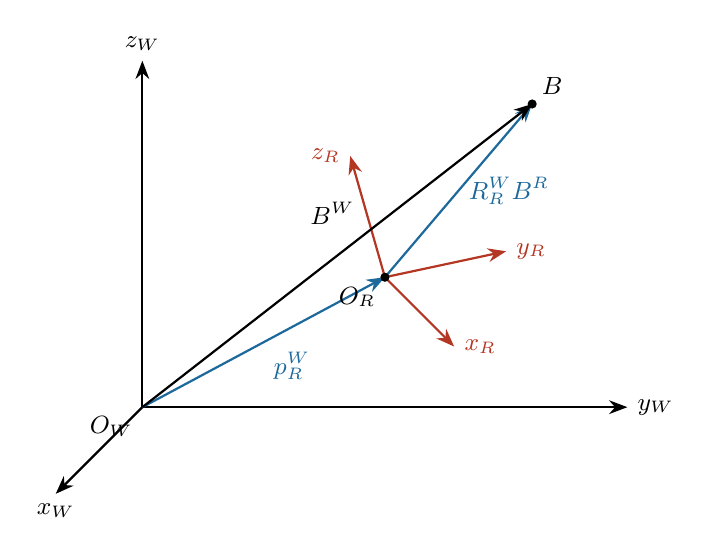
\begin{tikzpicture}[scale=1.1]
\coordinate (O) at (0,0);
\coordinate (R) at (2.8,1.5);
\coordinate (B) at (4.5,3.5);
\draw[axis] (O)--(-1,-1) node[below] {$x_W$};
\draw[axis] (O)--(5.6,0) node[right] {$y_W$};
\draw[axis] (O)--(0,4) node[above] {$z_W$};
\draw[axis,robotframe] (R)--(3.6,.7) node[right] {$x_R$};
\draw[axis,robotframe] (R)--(4.2,1.8) node[right] {$y_R$};
\draw[axis,robotframe] (R)--(2.4,2.9) node[left] {$z_R$};
\draw[axis,sensorframe] (O)--(R) node[midway,below right] {$p_R^W$};
\draw[axis,sensorframe] (R)--(B) node[midway,right] {$R_R^W B^R$};
\draw[axis] (O)--(B) node[pos=.57,above left] {$B^W$};
\fill (R) circle(1.5pt) node[below left] {$O_R$};
\fill (B) circle(1.5pt) node[above right] {$B$};
\node[below left] at (O) {$O_W$};
\end{tikzpicture}

\caption{Spatial coordinate transformation. The displacement from $O_W$ to
$B$ is the sum of the displacement to $O_R$ and the displacement from $O_R$
to $B$. All three labeled displacement vectors use world components.
The perspective sketch illustrates the geometry, not the numerical example.}
\label{fig:l05-geometry}
\end{figure}

The dimensions provide a useful check:
\[
 \underbrace{B^W}_{3\times1}
 =\underbrace{R_R^W}_{3\times3}\underbrace{B^R}_{3\times1}
 +\underbrace{p_R^W}_{3\times1}.
\]
Rotation alone maps direction vectors between frames. Translation is required
for point coordinates because the two origins can differ. For example,
subtracting the transformed coordinates of two points cancels $p_R^W$,
leaving only the rotation of their displacement.

\subsection{Worked example}
Take
\[
 p_R^W=\begin{bmatrix}1\\0\\2\end{bmatrix},\qquad
 B^R=\begin{bmatrix}2\\0\\1\end{bmatrix},\qquad
 R_R^W=R_z(\pi/4)=\begin{bmatrix}c&-c&0\\c&c&0\\0&0&1\end{bmatrix},
 \quad c=\frac{\sqrt2}{2}.
\]
The rotation is about $z$, chosen to simplify the arithmetic; the transformation
law applies equally to a general spatial rotation. Substitution gives
\begin{equation}
 B^W=\begin{bmatrix}2c\\2c\\1\end{bmatrix}
      +\begin{bmatrix}1\\0\\2\end{bmatrix}
     =\begin{bmatrix}1+\sqrt2\\\sqrt2\\3\end{bmatrix}.
 \label{eq:l05-example}
\end{equation}

\section{The reverse coordinate transformation}
To recover the coordinates in $R$, first subtract the origin's world position
and then apply the inverse rotation:
\begin{equation}
 \boxed{B^R=(R_R^W)\trans(B^W-p_R^W).}
 \label{eq:l05-reverse}
\end{equation}
The order matters. The subtraction takes place in $W$; the transpose then
converts that displacement into $R$ components. For the example,
\[
 B^R=\begin{bmatrix}c&c&0\\-c&c&0\\0&0&1\end{bmatrix}
 \begin{bmatrix}\sqrt2\\\sqrt2\\1\end{bmatrix}
 =\begin{bmatrix}2\\0\\1\end{bmatrix}.
\]

\section{Homogeneous transformations in space}
Introduce homogeneous point coordinates by appending a one:
\[
 \widetilde B^R=\begin{bmatrix}B^R\\1\end{bmatrix}\in\R^4.
\]
The spatial homogeneous transformation is
\begin{equation}
 H_R^W=\begin{bmatrix}R_R^W&p_R^W\\0_{1\times3}&1\end{bmatrix}
 \in\R^{4\times4},\qquad
 \boxed{\widetilde B^W=H_R^W\widetilde B^R.}
 \label{eq:l05-homogeneous}
\end{equation}
The lower-left block contains three zeros. Block multiplication reproduces
Equation~\eqref{eq:l05-affine} in the first three rows and preserves the final
one. Lines drawn between blocks are visual guides, not extra operations.

For the worked example,
\[
 H_R^W=\begin{bmatrix}
 c&-c&0&1\\c&c&0&0\\0&0&1&2\\0&0&0&1
 \end{bmatrix},\qquad
 H_R^W\begin{bmatrix}2\\0\\1\\1\end{bmatrix}
 =\begin{bmatrix}1+\sqrt2\\\sqrt2\\3\\1\end{bmatrix}.
\]
The last entry is a consistency check for this representation of a point under
a rigid transformation. A direction vector is instead augmented with zero;
then multiplication rotates the direction without adding a translation.

\subsection{Composition follows the frame chain}
The advantage of homogeneous coordinates remains the same as in the planar
case. For an intermediate frame $R$ and a sensor frame $S$,
\begin{equation}
 H_S^W=H_R^W H_S^R.
 \label{eq:l05-composition}
\end{equation}
Expanding the blocks gives
\[
 H_S^W=\begin{bmatrix}
 R_R^W R_S^R&R_R^W p_S^R+p_R^W\\0_{1\times3}&1
 \end{bmatrix}.
\]
Thus the rotation composes by multiplication, while the sensor-origin
displacement must be rotated into $W$ before adding $p_R^W$. The rightmost
map acts first: $S\to R\to W$. This is the spatial version of the earlier
frame-chain rule.

\section{Inverting a homogeneous transformation}
Rearranging Equation~\eqref{eq:l05-reverse} separates the reverse rotation
and translation:
\[
 B^R=(R_R^W)\trans B^W-(R_R^W)\trans p_R^W.
\]
Consequently,
\begin{equation}
 \boxed{H_W^R=(H_R^W)^{-1}
 =\begin{bmatrix}(R_R^W)\trans&-(R_R^W)\trans p_R^W\\0_{1\times3}&1\end{bmatrix}.}
 \label{eq:l05-inverse}
\end{equation}
This uses the structure of a rigid transformation instead of a general
$4\times4$ inversion. Multiplying the original and inverse blocks gives
$R_R^W(R_R^W)\trans=I_3$ and translation
$-R_R^W(R_R^W)\trans p_R^W+p_R^W=0$, verifying the result.

\subsection{Why reversing the translation requires a rotation}
The upper-right block of the inverse is
\begin{equation}
 \boxed{p_W^R=-(R_R^W)\trans p_R^W.}
 \label{eq:l05-inverse-position}
\end{equation}
Geometrically, the displacement from $O_R$ to $O_W$ is opposite to the
displacement from $O_W$ to $O_R$. However, $p_R^W$ uses world components,
whereas $p_W^R$ uses robot components. Negating the former reverses the
physical displacement but leaves its components expressed in $W$.
The transpose is needed to express them in $R$.

In the example,
\[
 p_W^R=-\begin{bmatrix}c&c&0\\-c&c&0\\0&0&1\end{bmatrix}
 \begin{bmatrix}1\\0\\2\end{bmatrix}
 =\begin{bmatrix}-c\\c\\-2\end{bmatrix},
\]
which differs from $-p_R^W=[-1\;0\;-2]\trans$. The full reverse transformation is
\[
 H_W^R=\begin{bmatrix}c&c&0&-c\\-c&c&0&c\\0&0&1&-2\\0&0&0&1\end{bmatrix}.
\]
Applying it to $[1+\sqrt2\;\sqrt2\;3\;1]\trans$ returns
$[2\;0\;1\;1]\trans$, as required.

\section{What rounding changes}
Replacing $c=\sqrt2/2$ by $0.7$ makes the forward calculation especially
simple. Denote the resulting approximate rotation by
\[
 \widehat R=\begin{bmatrix}.7&-.7&0\\.7&.7&0\\0&0&1\end{bmatrix}.
\]
With the same translation and input point, it gives
\[
 \widehat B^W=\widehat R B^R+p_R^W
 =\begin{bmatrix}2.4\\1.4\\3\end{bmatrix}.
\]
If we now use the transpose as though it were the inverse, the return
calculation produces
\[
 \widehat R\trans(\widehat B^W-p_R^W)
 =\begin{bmatrix}.7&.7&0\\-.7&.7&0\\0&0&1\end{bmatrix}
 \begin{bmatrix}1.4\\1.4\\1\end{bmatrix}
 =\begin{bmatrix}1.96\\0\\1\end{bmatrix}.
\]
The discrepancy has a precise explanation:
\begin{equation}
 \widehat R\trans\widehat R=\operatorname{diag}(.98,.98,1)\ne I_3.
 \label{eq:l05-roundoff}
\end{equation}
After rounding, $\widehat R$ is not an exact rotation matrix, and its transpose
is not its exact inverse. The return calculation scales the first two input
components by $0.98$. The exact radical form returns the original point
without this error.

This deliberately coarse rounding illustrates why orthogonality matters.
Using the actual algebraic inverse of $\widehat R$ would reverse its own
forward map exactly in exact arithmetic, but that map would still fail to be
a rigid rotation. In numerical work, keep adequate precision and monitor the
rotation constraints rather than assuming that a matrix labeled as a rotation
automatically satisfies them.

\section{Position, orientation, and pose}
\emph{Position} specifies the location of a chosen body-fixed origin relative
to a reference frame. In space it has three degrees of freedom.
\emph{Orientation} specifies how the body-fixed axes are aligned relative
to the reference axes and has three more continuous degrees of freedom.
Together, position and orientation define the body's \emph{pose}.
An unconstrained rigid body in space therefore has six degrees of freedom.

The number of stored components need not equal the number of degrees of
freedom. A rotation matrix contains nine entries subject to six independent
orthonormality constraints, with determinant $+1$ selecting proper rotations.
A unit quaternion has four components subject to one norm constraint.
Both describe three continuous degrees of freedom. RPY angles use three
parameters directly, with the singularity and nonuniqueness discussed in
Chapter~\ref{chap:lecture04}.

\begin{center}
\renewcommand{\arraystretch}{1.25}
\begin{tabular}{lll}
\toprule
Pose representation & Stored entries & Main condition or limitation\\
\midrule
$H_R^W$ & 16 & Rigid-transform block structure\\
Position and RPY & 6 & Angle ranges and singularities\\
Position and quaternion & 7 & Unit quaternion; $q$ and $-q$ equivalent\\
\bottomrule
\end{tabular}
\end{center}

For example, two vector representations are
\[
 \begin{bmatrix}p_R^W\\\varphi_R^W\\\theta_R^W\\\psi_R^W\end{bmatrix}
 \in\R^6,\qquad
 \begin{bmatrix}p_R^W\\q_R^W\end{bmatrix}\in\R^7,
\]
where $q_R^W$ represents the same orientation as $R_R^W$ under the
scalar-first convention. Stacking the components does not make pose
composition ordinary vector addition. To combine poses, use the appropriate
rotation and translation rules, conveniently encoded by homogeneous matrices.

Once both the position and orientation of a body-fixed frame are specified,
the locations of all points fixed to that rigid body follow from their
constant coordinates in that frame. This is why a single pose describes
the placement of the entire rigid body.

\clearpage
\section{Additional exercises}
Use right-handed frames and exact values unless rounding is explicitly requested.
\begin{enumerate}
\item \textbf{A spatial point transformation.}
Let $R_R^W=R_x(\pi/2)$, $p_R^W=[1\;-2\;3]\trans$, and
$B^R=[2\;1\;0]\trans$. Find $B^W$ and recover $B^R$ using the reverse map.

\item \textbf{Homogeneous form.}
Build $H_R^W$ for Exercise 1 and use it to transform $\widetilde B^R$.
Build $(H_R^W)^{-1}$ using its blocks and verify that their product is $I_4$.

\item \textbf{Reversing a displacement.}
For $R_R^W=R_z(\pi/2)$ and $p_R^W=[2\;1\;3]\trans$, compute $p_W^R$.
Compare it with $-p_R^W$ and explain the frame difference. Verify that
$R_R^W p_W^R+p_R^W=0$.

\item \textbf{A sensor frame.}
Suppose $R_R^W=R_z(\pi/2)$, $p_R^W=[1\;0\;2]\trans$,
$R_S^R=I_3$, and $p_S^R=[1\;0\;1]\trans$.
Find $H_S^W$ and the world coordinates of $B^S=[0\;2\;0]\trans$.
Check your result by transforming first to $R$ and then to $W$.

\item \textbf{Points and directions.}
Using the transformation in Exercise 1, transform the points
$A^R=[0\;0\;0]\trans$ and $B^R=[2\;1\;0]\trans$.
Show that $B^W-A^W=R_R^W(B^R-A^R)$.
Explain why a homogeneous direction uses a final zero instead of a one.

\item \textbf{Rounding and orthogonality.}
Replace $c$ in the worked example by $a=0.707$.
Derive $\widehat R\trans\widehat R=\operatorname{diag}(2a^2,2a^2,1)$.
Find the result of the forward map followed by the transpose-based reverse
map for $B^R=[2\;0\;1]\trans$, and compare with the $a=0.7$ result.

\item \textbf{Components versus degrees of freedom.}
Explain why position plus a unit quaternion stores seven numbers but describes
six continuous degrees of freedom. Normalize $q=[2\;0\;0\;2]\trans$.
Use Appendix~\ref{app:rotation-conversions} to find its rotation matrix,
then build a homogeneous transformation with position $[1\;0\;2]\trans$.
\end{enumerate}

% Opening from lecture 05; extend with subsequent lectures on sensing.
\chapter{Robot systems and sensing}
\label{chap:lecture06}

Reference frames and transformations describe where a robot and the objects
around it are located. A robot must also obtain information about those objects,
decide what to do, and produce physical motion. These activities connect the
geometric tools of the preceding chapters to the operation of a robot system.

\section{Sensing, processing, and action}
A useful working description of a robot is an intelligent interconnection
between sensing and action. Sensors collect measurements; computation uses
those measurements to select actions; actuators carry out the actions.
The resulting interaction with the environment produces new measurements,
closing a feedback loop.

\begin{figure}[htbp]
\centering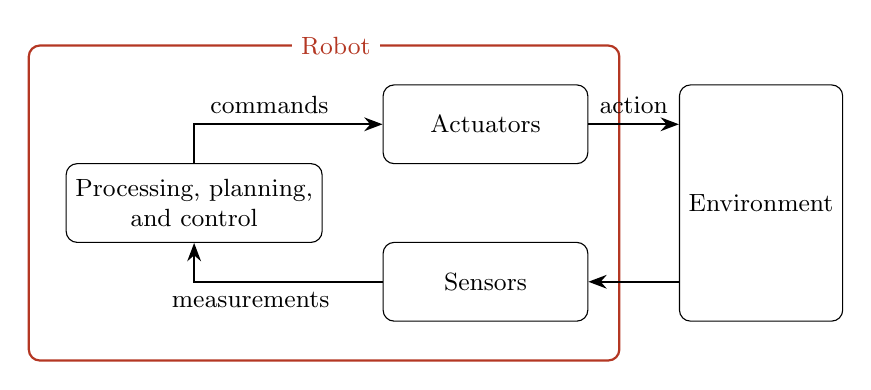
\begin{tikzpicture}[box/.style={draw,rounded corners,align=center,minimum height=1cm,minimum width=2.6cm}]
\draw[rounded corners,robotframe,thick] (-2.1,-2) rectangle (5.4,2);
\node[robotframe,fill=white] at (1.8,2) {Robot};
\node[box] (I) at (0,0) {Processing, planning,\\and control};
\node[box] (A) at (3.7,1) {Actuators};
\node[box] (S) at (3.7,-1) {Sensors};
\node[box,minimum width=2cm,minimum height=3cm] (E) at (7.2,0) {Environment};
\draw[axis] (I.north) |- (A.west) node[pos=.7,above] {commands};
\draw[axis] (S.west) -| (I.south) node[pos=.35,below] {measurements};
\draw[axis] (A.east)--(A.east -| E.west) node[midway,above] {action};
\draw[axis] (S.east -| E.west)--(S.east);
\end{tikzpicture}

\caption{A functional view of a robot interacting with its environment.
The robot boundary contains sensors, actuators, and the hardware and software
that process measurements and generate commands.}
\label{fig:l06-components}
\end{figure}

\section{Sensors and the environment}
The \emph{environment} includes the objects, surfaces, and people with which
the robot interacts. A camera measures incoming light, a microphone responds
to pressure variations, and a contact sensor detects physical contact.
Sensors may also measure the robot's own state; sensing is not limited to
observing external objects.

A measurement is not yet an interpretation of the scene. An image records
light arriving at the camera; identifying an object and estimating its
location require processing that image. Likewise, a contact measurement
indicates an interaction at a surface but does not by itself describe the
entire surrounding space. Each type of sensor provides particular information
that the robot must interpret in relation to its task.

The coordinate transformations developed earlier enter at this point. An
object located in a sensor frame may need to be expressed in a robot frame
to determine whether it is within reach, or in a world frame to plan motion.
The physical object is the same; the coordinate description is chosen to
support the calculation being performed.

\section{Actuators and physical interaction}
\emph{Actuators} produce physical action, for example by driving wheels or
moving a manipulator. Wheel-driven motion depends on forces exchanged with
the supporting surface. An action may change the environment, the robot's
pose relative to it, or both.

The distinction between sensing and action is a useful functional one:
sensors provide measurements, whereas actuators produce physical effects.
A motor command can turn a wheel or move a joint, but the resulting motion
also depends on the mechanism and its interaction with the surroundings.
Moving a mobile robot changes what its sensors observe, even when the objects
in the environment remain fixed in the world frame.

\section{Connecting measurements to commands}
The connection between sensing and action includes both computing hardware
and software. It may involve interpreting measurements, estimating where
objects are, selecting a plan, and producing individual actuator commands.
Here, ``intelligent'' does not require a neural network or machine learning:
explicit algorithms and feedback control can also provide this connection.

The central block in Figure~\ref{fig:l06-components} therefore represents
several possible levels of computation. A high-level decision might be to
approach an object. More detailed decisions specify how to move, and the
commands sent to the actuators must ultimately specify actions that the
hardware can execute. All of these functions belong to the connection
between measurements and physical action, even when they run in different
programs or on different processors.

The enclosing boundary in the diagram is also important: the robot includes
the sensors and actuators as well as the computing hardware and software.
The central block alone is not the entire robot. The arrows trace a loop
through the environment: an action changes the physical situation, sensors
measure the resulting situation, and computation can use those measurements
to decide the next action.

\subsection{Example: reaching an object}
Suppose a robot must grasp an object that is initially beyond its reach.
Sensor measurements first support an estimate of the object's location.
The robot must then determine that it needs to move closer, choose an approach,
and command its motion before extending the manipulator and closing the gripper.
A high-level objective thus becomes a sequence of physical actions, with
measurements available to check progress and adjust the commands.

Consider the distinction between the decisions involved. Recognizing the
object answers what the robot should interact with. Estimating its position
answers where it is. Comparing that position with the robot's reach determines
whether the base must move first. Planning selects a sequence of motions,
and control turns those motions into actuator commands. These decisions
serve the same task but require different information and computations.

After the robot approaches, the object's coordinates relative to the robot
have changed. New measurements can update its estimated location before the
grasp. This illustrates why sensing and action are connected repeatedly:
the robot does not merely observe once and then execute an unrelated motion.

\appendix
\chapter{Rotation representation conversions}
\label{app:rotation-conversions}
\begingroup
\small

This reference collects conversions between rotation matrices,
roll--pitch--yaw (RPY) angles, and unit quaternions. The matrix and angle
conventions agree with Chapter~\ref{chap:lecture04}, which introduces the
practical use of unit quaternions.

\section*{Conventions}
All frames are right-handed, vectors are columns, and
\[
 R=R_z(\psi)R_y(\theta)R_x(\varphi)\in SO(3),\qquad
 SO(3)=\{R\in\R^{3\times3}:R\trans R=I_3,\ \det R=1\}.
\]
The angles are roll $\varphi$, pitch $\theta$, and yaw $\psi$, with principal
ranges $\varphi,\psi\in(-\pi,\pi]$ and $\theta\in[-\pi/2,\pi/2]$.
Quaternions use the scalar-first convention
\[
 q=\begin{bmatrix}q_w&q_x&q_y&q_z\end{bmatrix}\trans,\qquad
 q_w^2+q_x^2+q_y^2+q_z^2=1.
\]
The signs in the formulas below specify the quaternion convention; a different
component order must be converted before applying them. The quaternions $q$
and $-q$ represent the same rotation. Write $c_a=\cos a$ and $s_a=\sin a$.
The function $\operatorname{atan2}(y,x)$ takes its arguments in that order.

\section*{RPY angles to a rotation matrix}
\[
 R=\begin{bmatrix}
 c_\psi c_\theta & c_\psi s_\theta s_\varphi-s_\psi c_\varphi & c_\psi s_\theta c_\varphi+s_\psi s_\varphi\\
 s_\psi c_\theta & s_\psi s_\theta s_\varphi+c_\psi c_\varphi & s_\psi s_\theta c_\varphi-c_\psi s_\varphi\\
 -s_\theta & c_\theta s_\varphi & c_\theta c_\varphi
 \end{bmatrix}.
\]

\section*{Rotation matrix to RPY angles}
For $R=[r_{ij}]$ and $|\theta|<\pi/2$,
the angles are recovered by the formulas below. At $\theta=\pm\pi/2$, yaw
and roll are not separately determined; a singular-case convention is required.
In particular, $\operatorname{atan2}(0,0)$ has no unique geometric meaning.
\[
 \begin{aligned}
 \varphi&=\operatorname{atan2}(r_{32},r_{33}),\\
 \theta&=\operatorname{atan2}\!\left(-r_{31},\sqrt{r_{32}^2+r_{33}^2}\right),\\
 \psi&=\operatorname{atan2}(r_{21},r_{11}).
 \end{aligned}
\]
\clearpage
\section*{Unit quaternion to a rotation matrix}
\[
 R=\begin{bmatrix}
 1-2(q_y^2+q_z^2)&2(q_xq_y-q_wq_z)&2(q_xq_z+q_wq_y)\\
 2(q_xq_y+q_wq_z)&1-2(q_x^2+q_z^2)&2(q_yq_z-q_wq_x)\\
 2(q_xq_z-q_wq_y)&2(q_yq_z+q_wq_x)&1-2(q_x^2+q_y^2)
 \end{bmatrix}.
\]
This expression assumes a unit quaternion. Normalize a nonzero quaternion
before using it; a zero quaternion does not describe an orientation.

\section*{RPY angles to a unit quaternion}
Using the same intrinsic Z--Y--X convention,
\[
 \begin{aligned}
 q_w&=c_{\varphi/2}c_{\theta/2}c_{\psi/2}
       +s_{\varphi/2}s_{\theta/2}s_{\psi/2},\\
 q_x&=s_{\varphi/2}c_{\theta/2}c_{\psi/2}
       -c_{\varphi/2}s_{\theta/2}s_{\psi/2},\\
 q_y&=c_{\varphi/2}s_{\theta/2}c_{\psi/2}
       +s_{\varphi/2}c_{\theta/2}s_{\psi/2},\\
 q_z&=c_{\varphi/2}c_{\theta/2}s_{\psi/2}
       -s_{\varphi/2}s_{\theta/2}c_{\psi/2}.
 \end{aligned}
\]

\section*{Unit quaternion to RPY angles}
Away from the pitch singularities,
\[
 \begin{aligned}
 \varphi&=\operatorname{atan2}\!\left(2(q_wq_x+q_yq_z),\,
                      1-2(q_x^2+q_y^2)\right),\\
 \theta&=\arcsin\!\left(2(q_wq_y-q_zq_x)\right),\\
 \psi&=\operatorname{atan2}\!\left(2(q_wq_z+q_xq_y),\,
                      1-2(q_y^2+q_z^2)\right).
 \end{aligned}
\]
For a normalized quaternion, the exact argument of $\arcsin$ lies in $[-1,1]$.
In floating-point arithmetic, clamp small roundoff excursions to that interval
before evaluating $\arcsin$. This does not resolve the pitch singularity,
nor does it replace checking the quaternion's normalization.

\clearpage
\section*{Rotation matrix to a unit quaternion}
One conversion branch chooses $q_w\ge0$:
\[
 \begin{aligned}
 q_w&=\tfrac12\sqrt{1+r_{11}+r_{22}+r_{33}},\\
 q_x&=\frac{r_{32}-r_{23}}{4q_w},\qquad
 q_y=\frac{r_{13}-r_{31}}{4q_w},\qquad
 q_z=\frac{r_{21}-r_{12}}{4q_w}.
 \end{aligned}
\]
\textbf{This branch requires $q_w\ne0$.} It fails for an exact half-turn
and is numerically sensitive near a half-turn. A robust implementation selects
a branch whose denominator is large. The following equivalent identities
provide the alternative branches:
\[
 \begin{aligned}
 4q_w^2&=1+r_{11}+r_{22}+r_{33},&
 4q_x^2&=1+r_{11}-r_{22}-r_{33},\\
 4q_y^2&=1-r_{11}+r_{22}-r_{33},&
 4q_z^2&=1-r_{11}-r_{22}+r_{33}.
 \end{aligned}
\]
Choose a largest squared component, assign its positive square root, and
recover the other components from
\[
 \begin{aligned}
 4q_wq_x&=r_{32}-r_{23},&4q_xq_y&=r_{12}+r_{21},\\
 4q_wq_y&=r_{13}-r_{31},&4q_xq_z&=r_{13}+r_{31},\\
 4q_wq_z&=r_{21}-r_{12},&4q_yq_z&=r_{23}+r_{32}.
 \end{aligned}
\]
For example, if $q_x$ is chosen, divide the identities for $q_wq_x$,
$q_xq_y$, and $q_xq_z$ by $4q_x$ to obtain $q_w,q_y,q_z$. For a valid
rotation at least one component has magnitude at least $1/2$. Normalize
the resulting quaternion to remove small numerical drift. These formulas
assume the input is a proper rotation matrix; they do not repair an arbitrary matrix.
\par
\endgroup

\end{document}
